\documentclass[11pt,a4paper]{article}

% Overleaf / pdfLaTeX Standard Packages
\usepackage[utf8]{inputenc}
\usepackage[T1]{fontenc}
\usepackage[margin=1in]{geometry}
\usepackage{graphicx}
\usepackage{booktabs}
\usepackage{array}
\usepackage{tabularx}
\usepackage{multirow}
\usepackage{amsmath}
\usepackage{amssymb}
\usepackage{xcolor}
\usepackage{float}
\usepackage{caption}
\usepackage{enumitem}
\usepackage{fancyhdr}
\usepackage{titlesec}
\usepackage{microtype}
\usepackage{setspace}
\usepackage{url}
\usepackage[numbers,sort&compress]{natbib}
\usepackage[colorlinks=true,linkcolor=blue!60!black,citecolor=blue!60!black,urlcolor=blue!60!black]{hyperref}
\usepackage{doi}
\renewcommand{\doitext}{https://doi.org/}

% Graphics Path Configuration (Overleaf figures/ + local fallback)
\graphicspath{{figures/}{../../results/figures/}}

% Header and Footer Styling
\pagestyle{fancy}
\fancyhf{}
\fancyhead[L]{\small\textit{CSE477: Data Mining --- Group 10 Research Report}}
\fancyhead[R]{\small\textit{East West University}}
\fancyfoot[C]{\thepage}
\renewcommand{\headrulewidth}{0.5pt}
\renewcommand{\footrulewidth}{0.3pt}

% Section Title Formatting
\titleformat{\section}{\large\bfseries\color{blue!40!black}}{\thesection}{1em}{}
\titleformat{\subsection}{\normalsize\bfseries\color{blue!30!black}}{\thesubsection}{1em}{}
\titleformat{\subsubsection}{\small\bfseries}{\thesubsubsection}{1em}{}

\begin{document}

% ==============================================================================
% DEDICATED EAST WEST UNIVERSITY COVER PAGE
% ==============================================================================
\begin{titlepage}
    \centering
    \vspace*{0.5cm}
    
    % University Header & Optional Logo Hook
    {\LARGE \textbf{EAST WEST UNIVERSITY}}\\[0.25cm]
    {\large \textbf{Department of Computer Science and Engineering}}\\[0.6cm]
    
    % \includegraphics[width=3.2cm]{ewu_logo.png}\\[0.5cm]
    
    \vspace{0.8cm}
    \rule{\linewidth}{1.2pt}\\[0.4cm]
    {\Large \textbf{Surviving Imperfect Data: A Multi-Dimensional Robustness Stress Test of Data Mining Pipelines on Morphological Dry Bean Features}}\\[0.2cm]
    \rule{\linewidth}{1.2pt}
    
    \vspace{1.0cm}
    {\large \textbf{Course:} CSE477 --- Data Mining \quad \textbf{Section:} 4}\\[0.2cm]
    {\large \textbf{Semester:} Fall 2026}\\[0.4cm]
    {\large \textbf{Assigned Research Theme:}}\\[0.15cm]
    {\large \textbf{Group 10 --- ``The Data Mining Stress Test''}}\\[0.1cm]
    {\textit{(How Much Can a Data-Mining Model Survive?)}}\\[1.2cm]
    
    % Framed Submission Metadata Box
    \noindent\fbox{%
        \parbox{0.92\linewidth}{%
            \vspace{0.25cm}
            \textbf{\large Submitted By (Group 10):}\\[0.2cm]
            \begin{tabular}{ll}
                \textbf{Syed Zubayear Bin Khaled} & ID: \texttt{2023-2-60-107} \\
                \textbf{Md. Arifur Rahman Shihab} & ID: \texttt{2023-2-60-176} \\
            \end{tabular}\\[0.4cm]
            \textbf{\large Submitted To:}\\[0.2cm]
            \begin{tabular}{l}
                \textbf{Sanzana Karim Lora} \\
                Lecturer, Department of Computer Science and Engineering \\
                East West University \\
            \end{tabular}\\[0.25cm]
        }%
    }
    
    \vfill
    {\small \textbf{Public Artifact Repository:} \url{https://github.com/zubayearBK/cse477-dry-bean-stress-test}}\\[0.15cm]
    {\small Date of Submission: Fall 2026}
    \vspace*{0.5cm}
\end{titlepage}

% ==============================================================================
% FRONT MATTER
% ==============================================================================
\newpage
\pagenumbering{roman}
\tableofcontents
\newpage
\listoffigures
\vspace{0.8cm}
\listoftables
\newpage

% ==============================================================================
% ABSTRACT & KEYWORDS
% ==============================================================================
\pagenumbering{arabic}
\setcounter{page}{1}

\begin{center}
    {\Large \textbf{Surviving Imperfect Data: A Multi-Dimensional Robustness Stress Test of Data Mining Pipelines on Morphological Dry Bean Features}}\\[0.4cm]
    {\large Syed Zubayear Bin Khaled \quad and \quad Md. Arifur Rahman Shihab}\\[0.2cm]
    {\small Department of Computer Science and Engineering, East West University, Dhaka, Bangladesh}\\[0.4cm]
\end{center}

\begin{abstract}
Real-world data mining pipelines in agricultural computer vision frequently fail when deployed on noisy, degraded telemetry, despite exhibiting high accuracy on pristine laboratory benchmarks. In this paper, we present a systematic empirical investigation and multi-dimensional robustness stress test evaluating how data mining algorithms survive controlled data corruption. Using the benchmark UCI Dry Bean dataset ($N = 13{,}611$, cleaned to $N = 13{,}543$ grains across seven commercial cultivars after deduplicating $68$ records), we analyze $16$ continuous morphological features across similarity metrics, unsupervised clustering ($k$-Means, Hierarchical Ward, DBSCAN), supervised classification (Decision Trees, Rule-Based Classifiers, Gaussian Naïve Bayes, $k$-Nearest Neighbors), and discretized FP-Growth association rule mining. We then subject these pipelines to four controlled degradation regimes: Missing Completely at Random (MCAR) injection ($0\%$--$30\%$), extreme sensor outlier corruption ($0\%$--$20\%$ at $+8\sigma$), normalization sensitivity under clean and corrupted distributions, and collinearity/dimensionality reduction (pruned 8-feature subset and PCA). Our findings reveal that: (1) unscaled raw Euclidean distance collapses into a one-dimensional pixel-count sort due to a $75.5\text{M}\times$ scale disparity between Area and ShapeFactor2, dropping neighbor class purity by $\Delta = -0.2498$; (2) Decision Trees exhibit remarkable invariance to extreme $+8\sigma$ outliers (Macro-F1 drops by only $1.10$ percentage points, a $1.19\%$ relative drop at $20\%$ corruption), whereas $k$-Means ARI collapses catastrophically from $0.6669$ to $0.2427$; and (3) pruning collinear features directly improves Gaussian Naïve Bayes Macro-F1 from $0.9072$ to $0.9208$ by restoring conditional independence. We conclude with actionable architecture guidelines for robust agricultural sorting systems.
\end{abstract}

\noindent\textbf{Keywords:} Data Mining Robustness, Stress Testing, Agricultural Computer Vision, Morphological Feature Extraction, Model Degradation Trajectories, Dry Bean Classification.

\vspace{0.5cm}

% ==============================================================================
% SECTION 1: INTRODUCTION
% ==============================================================================
\section{Introduction}
\label{sec:introduction}

In modern automated agriculture, high-throughput machine vision systems are increasingly deployed to inspect, grade, and sort bulk grain harvests into commercial botanical cultivars~\citep{koklu2020multiclass}. While machine learning and data mining models routinely achieve classification accuracies exceeding $90\%$ on curated, noise-free laboratory benchmarks, their performance in industrial sorting facilities frequently collapses~\citep{han2022datamining,tan2019introduction}. In operational grain elevators and processing plants, optical segmentation pipelines suffer from lens dust, fluctuating illumination, partial grain occlusions, missing sensor telemetry, optical sensor glitches, and calibration drift. 

Standard academic investigations prioritize optimizing accuracy on pristine benchmarks, tacitly assuming that the training and operational test distributions remain clean and identical. This paradigm obscures a critical engineering question: \textit{Under what specific data-quality degradations do classical data mining algorithms fail, which methods fail gracefully, which collapse catastrophically, and why?}

As \textbf{Group 10 (``The Data Mining Stress Test'')}, our research mandate departs from conventional accuracy chasing. We treat the benchmark UCI Dry Bean dataset~\citep{uci2020drybean,koklu2020multiclass} as a pristine scientific baseline ($100\%$ data quality) and systematically subject data mining pipelines to controlled, multi-dimensional data degradation. We formalize this inquiry around four primary Stress-Test Research Questions (SRQ1--SRQ4) alongside four core Data Mining Research Questions (RQ1--RQ4):

\subsection{Research Questions}
\label{subsec:research_questions}

\begin{itemize}[leftmargin=1.5em]
    \item \textbf{SRQ1 (Missing Data Tolerance):} How rapidly do unsupervised clustering quality (Silhouette, ARI) and supervised classification performance (Macro-F1, Accuracy) degrade under $5\%$, $10\%$, $20\%$, and $30\%$ Missing Completely at Random (MCAR) corruption, and how effectively do Median versus $k$-NN imputation strategies buffer this collapse?
    \item \textbf{SRQ2 (Outlier and Noise Vulnerability):} To what extent do injected extreme sensor outliers ($5\%$, $10\%$, $20\%$ at $+8\sigma$) distort centroid-based clustering ($k$-Means) and distance-based classification ($k$-NN) compared to density-based (DBSCAN), hierarchical (Ward), tree-based (Decision Tree), and probabilistic (Gaussian Naïve Bayes) paradigms?
    \item \textbf{SRQ3 (Scale and Normalization Sensitivity):} Given that raw morphological feature ranges span seven orders of magnitude ($75.5\text{M}\times$ scale disparity), how drastically do Min-Max, Z-score, and RobustScaler alter nearest-neighbor neighborhoods, clustering geometry, and model resilience under outlier contamination?
    \item \textbf{SRQ4 (Dimensionality and Collinearity Stress):} In the presence of extreme geometric collinearity (pairwise $r > 0.98$, maximum VIF $= 317{,}671.59$), does removing redundant features or applying PCA improve model robustness, or does aggressive compression degrade discrimination among morphologically similar cultivars?
    \item \textbf{RQ1 (Dominant Morphological Patterns):} What are the primary latent physical axes governing dry bean seed morphology?
    \item \textbf{RQ2 (Most Informative Attributes):} Which geometric and derived shape factors provide the highest mutual information and class separability?
    \item \textbf{RQ3 (Meaningful Natural Groupings and Overlaps):} What clusters emerge naturally from unsupervised geometry, and where do cultivar boundaries overlap?
    \item \textbf{RQ4 (Optimal Data Mining Architecture):} Which algorithmic paradigm demonstrates the highest structural resilience for agricultural sorting under degradation?
\end{itemize}

\subsection{Key Contributions}
\label{subsec:contributions}

The primary contributions of this paper are summarized as follows:
\begin{enumerate}[leftmargin=1.5em]
    \item \textbf{End-to-End Baseline Benchmark:} We establish a reproducible data mining baseline spanning distance metric analysis, unsupervised clustering ($k$-Means, Hierarchical Ward, DBSCAN), supervised classification (Decision Trees, Interpretable Rule Classifiers, Gaussian Naïve Bayes, $k$-NN), and discretized FP-Growth Class Association Rules.
    \item \textbf{Quantitative Scale Distortion Proof:} We prove mathematically and empirically that raw Euclidean distance collapses into a one-dimensional pixel-count sort due to \texttt{Area} dominance, causing a $\Delta = -0.2498$ drop in nearest-neighbor class purity.
    \item \textbf{Four Signature Robustness Curves:} We generate empirical degradation trajectories under Missingness, Outliers, Normalization Swaps, and Dimensionality Compression, mapping the exact breakdown thresholds of four distinct algorithmic paradigms.
    \item \textbf{Five High-Impact Discoveries:} We document five rigorously grounded findings, including the 100\% \texttt{BOMBAY} outlier paradox, Naïve Bayes performance inversion under collinearity pruning, and Decision Tree outlier immunity.
\end{enumerate}

% ==============================================================================
% SECTION 2: DATASET DESCRIPTION & TAXONOMY
% ==============================================================================
\section{Dataset Description and Taxonomy}
\label{sec:dataset_description}

The primary empirical foundation for this study is the UCI Dry Bean Dataset~\citep{uci2020drybean}, contributed by Koklu and Ozkan~\citep{koklu2020multiclass}. The dataset encapsulates 2D morphological feature vectors extracted from high-resolution digital computer vision images of registered Turkish dry bean grains. Table~\ref{tab:metadata} synthesizes the comprehensive dataset metadata specification.

\begin{table}[htbp]
    \centering
    \small
    \caption{UCI Dry Bean Dataset Metadata Specification.}
    \label{tab:metadata}
    \setlength{\tabcolsep}{5pt}
    \begin{tabularx}{\linewidth}{@{} >{\bfseries}l X @{}}
        \toprule
        Property & Specification / Metadata Details \\
        \midrule
        Dataset Name & Dry Bean Dataset \\
        Primary DOI / URI & \url{https://doi.org/10.24432/C50S4B} \\
        Primary Publication & Koklu and Ozkan (2020), \textit{Computers and Electronics in Agriculture}~\citep{koklu2020multiclass} \\
        Application Domain & Agricultural Computer Vision / High-Throughput Grain Inspection \\
        Data Object (1 Row) & One individual segmented dry bean grain silhouette \\
        Raw Record Count ($N$) & $13{,}611$ instances ($0$ missing values) \\
        Cleaned Record Count & $13{,}543$ instances ($68$ exact duplicate rows dropped) \\
        Dimensionality ($d$) & $17$ total attributes ($16$ continuous numerical features + $1$ nominal target class) \\
        Target Classes ($C = 7$) & \texttt{SEKER}, \texttt{BARBUNYA}, \texttt{BOMBAY}, \texttt{CALI}, \texttt{DERMASON}, \texttt{HOROZ}, \texttt{SIRA} \\
        Data Acquisition & Computer vision segmentation under controlled laboratory lighting \\
        \bottomrule
    \end{tabularx}
\end{table}

\subsection{Complete Attribute Taxonomy}
\label{subsec:attribute_taxonomy}

The 16 predictive features capture both absolute geometric dimensions and scale-invariant shape ratios. Table~\ref{tab:attributes} defines the complete mathematical taxonomy of all attributes, including their formal symbols, data-mining measurement types, mathematical formulations, and collinearity roles.

\begin{table}[htbp]
    \centering
    \footnotesize
    \caption{Comprehensive 17-Attribute Morphological Taxonomy and Mathematical Definitions.}
    \label{tab:attributes}
    \setlength{\tabcolsep}{3.5pt}
    \begin{tabularx}{\linewidth}{@{} c l c c >{\raggedright\arraybackslash}p{3.8cm} >{\raggedright\arraybackslash}X @{}}
        \toprule
        \textbf{\#} & \textbf{Attribute} & \textbf{Symbol} & \textbf{Type} & \textbf{Mathematical Definition} & \textbf{Physical Role \& Collinearity} \\
        \midrule
        1 & \texttt{Area} & $A$ & Discrete & Pixel count inside boundary & Core size; collinear with $C, E_d, P$ \\
        2 & \texttt{Perimeter} & $P$ & Cont. & Circumference pixel length & Core size metric; scale $\sim 10^3$ \\
        3 & \texttt{MajorAxisLength} & $L$ & Cont. & Longest ellipse axis & Primary elongation dimension \\
        4 & \texttt{MinorAxisLength} & $l$ & Cont. & Shortest axis perpendicular to $L$ & Grain width dimension \\
        5 & \texttt{AspectRation} & $K$ & Cont. & $K = L / l$ & Aspect ratio / elongation index \\
        6 & \texttt{Eccentricity} & $E_c$ & Cont. & $E_c = \sqrt{1 - (l/L)^2}$ & Non-linear elongation index \\
        7 & \texttt{ConvexArea} & $C$ & Discrete & Pixels in convex hull polygon & Nearly identical to Area ($r > 0.999$) \\
        8 & \texttt{EquivDiameter} & $E_d$ & Cont. & $E_d = \sqrt{4A / \pi}$ & Equivalent circle diameter \\
        9 & \texttt{Extent} & $E_x$ & Cont. & $E_x = A / (W_{bb} \cdot H_{bb})$ & Bounding-box fill efficiency \\
        10 & \texttt{Solidity} & $S$ & Cont. & $S = A / C$ & Boundary concavity ratio \\
        11 & \texttt{roundness} & $R$ & Cont. & $R = 4\pi A / P^2$ & Scale-invariant circularity metric \\
        12 & \texttt{Compactness} & $CO$ & Cont. & $CO = E_d / L$ & Circular compactness ratio \\
        13 & \texttt{ShapeFactor1} & $SF_1$ & Cont. & $SF_1 = L / A$ & Inverse size-elongation ($\sim 10^{-3}$) \\
        14 & \texttt{ShapeFactor2} & $SF_2$ & Cont. & $SF_2 = l / A$ & Inverse size-width ($\sim 10^{-3}$) \\
        15 & \texttt{ShapeFactor3} & $SF_3$ & Cont. & $SF_3 = A / (\frac{\pi}{4} L^2) = CO^2$ & Collinear with Compactness \\
        16 & \texttt{ShapeFactor4} & $SF_4$ & Cont. & $SF_4 = A / (\frac{\pi}{4} L \cdot l)$ & Convex ellipse ratio ($\approx 0.99$) \\
        17 & \texttt{Class} & $y$ & Nominal & Categorical label ($7$ classes) & Supervised ground truth; excluded in clustering \\
        \bottomrule
    \end{tabularx}
\end{table}

\subsection{Cultivar Prevalence and Class Imbalance}
\label{subsec:class_imbalance}

The dataset encompasses seven commercial dry bean cultivars with marked class imbalance. Table~\ref{tab:class_dist} details the frequency and percentage distribution of the cleaned dataset ($N = 13{,}543$).

\begin{table}[htbp]
    \centering
    \small
    \caption{Distribution of Dry Bean Cultivars in the Deduplicated Dataset ($N = 13{,}543$).}
    \label{tab:class_dist}
    \setlength{\tabcolsep}{5pt}
    \begin{tabularx}{\linewidth}{@{} l r r l X @{}}
        \toprule
        \textbf{Cultivar Class} & \textbf{Count ($n$)} & \textbf{Percentage} & \textbf{Role in Pipeline} & \textbf{Morphological Archetype} \\
        \midrule
        \texttt{DERMASON} & $3{,}546$ & $26.18\%$ & Majority Class & Small, rounded-oval grain \\
        \texttt{SIRA} & $2{,}636$ & $19.46\%$ & Majority Class & Medium-small oval grain \\
        \texttt{SEKER} & $2{,}027$ & $14.97\%$ & Intermediate & Highly spherical, compact grain \\
        \texttt{HOROZ} & $1{,}860$ & $13.73\%$ & Intermediate & Long, slender cylindrical grain \\
        \texttt{CALI} & $1{,}630$ & $12.04\%$ & Intermediate & Large, elongated kidney grain \\
        \texttt{BARBUNYA} & $1{,}322$ & $9.76\%$ & Intermediate & Large, broad speckled grain \\
        \texttt{BOMBAY} & $522$ & $3.85\%$ & Minority Class & Giant, massive white bean \\
        \midrule
        \textbf{Total Cleaned} & $\mathbf{13{,}543}$ & $\mathbf{100.00\%}$ & --- & Imbalance Ratio: $6.79:1$ \\
        \bottomrule
    \end{tabularx}
\end{table}

The dominant cultivar \texttt{DERMASON} ($3{,}546$ grains) outnumbers the minority cultivar \texttt{BOMBAY} ($522$ grains) by a ratio of $6.79:1$. This structural skew necessitates evaluating models using Macro-averaged F1-scores rather than raw overall accuracy, which would heavily disguise minority misclassifications. Figure~\ref{fig:class_dist} visualizes the class prevalence distribution.

\begin{figure}[htbp]
    \centering
    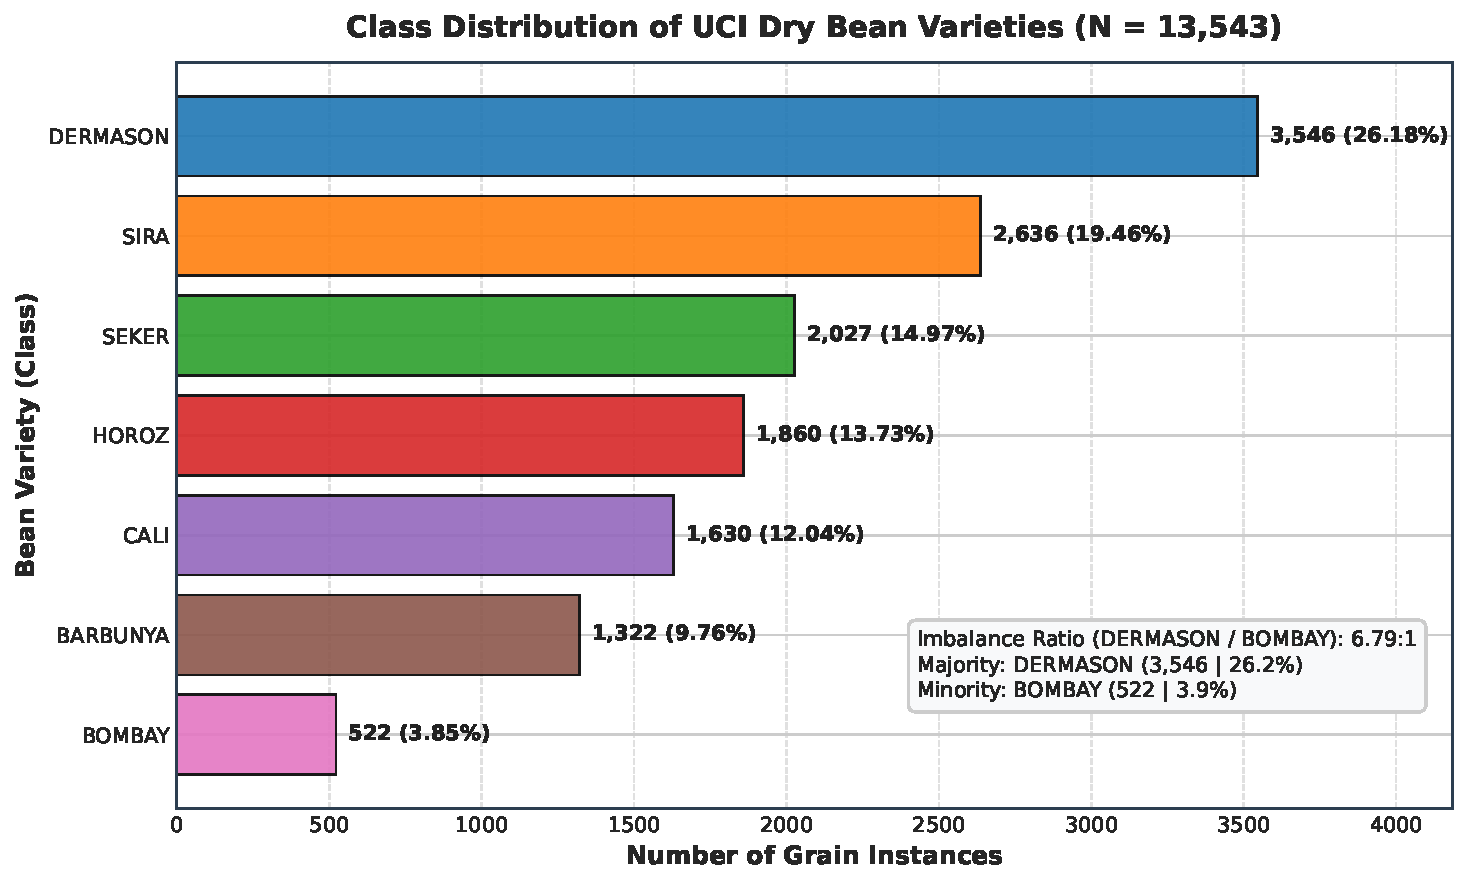
\includegraphics[width=0.82\linewidth]{fig02_class_distribution}
    \caption{Frequency distribution and relative class percentages across the seven dry bean cultivars in the cleaned dataset ($N = 13{,}543$).}
    \label{fig:class_dist}
\end{figure}

% ==============================================================================
% SECTION 3: DATA PREPROCESSING
% ==============================================================================
\section{Data Quality Audit and Preprocessing}
\label{sec:preprocessing}

To establish a rigorous baseline, we conduct a comprehensive data quality audit across six diagnostic dimensions: missingness, duplicate records, identifier leakage, naming anomalies, physical domain boundaries, and univariate outlier distributions.

\subsection{Data Quality Audit Findings}
\label{subsec:data_quality_audit}

Table~\ref{tab:data_quality} summarizes the results of the six-dimension data quality audit.

\begin{table}[htbp]
    \centering
    \small
    \caption{Six-Dimension Data Quality Audit and Resolution Actions.}
    \label{tab:data_quality}
    \setlength{\tabcolsep}{5pt}
    \begin{tabularx}{\linewidth}{@{} l >{\raggedright\arraybackslash}p{4.8cm} >{\raggedright\arraybackslash}X @{}}
        \toprule
        \textbf{Quality Dimension} & \textbf{Empirical Audit Finding} & \textbf{Resolution / Pipeline Action} \\
        \midrule
        \textbf{Missing Values} & Exactly $0$ missing cells across all $17$ columns ($100\%$ completeness). & Pristine baseline enables controlled MCAR injection experiments. \\
        \textbf{Duplicate Records} & Exactly $68$ duplicate records ($0.50\%$), all belonging to cultivar \texttt{HOROZ}. & Dropped programmatically ($N = 13{,}611 \to 13{,}543$) to prevent test-set leakage. \\
        \textbf{Identifier Leakage} & Zero surrogate keys, timestamps, or acquisition IDs present. & Confirmed; zero artificial leakage to target label. \\
        \textbf{Attribute Naming} & Historical typos in schema: \texttt{AspectRation} and lowercase \texttt{roundness}. & Mapped consistently to standard schema. \\
        \textbf{Domain Bounds} & All physical bounds valid: $A > 0, P > 0$, $E_c \in [0.219, 0.911], R \in [0.490, 0.991]$. & Confirmed $100\%$ valid within theoretical bounds. \\
        \textbf{Global Outliers} & $551$ instances ($4.07\%$) exceed $1.5\times\text{IQR}$ upper bound for \texttt{Area} ($99{,}031.25$). & Crucial discovery: $522/522$ \texttt{BOMBAY} beans ($100\%$) sit in outlier zone. Retained! \\
        \bottomrule
    \end{tabularx}
\end{table}

\subsection{The 100\% BOMBAY Outlier Paradox}
\label{subsec:bombay_outlier_paradox}

A critical empirical discovery emerged during the outlier audit: exactly $522$ out of the $551$ global IQR outliers on \texttt{Area} belong to the cultivar \texttt{BOMBAY}. In fact, \textbf{100.0\% of all \texttt{BOMBAY} beans in the entire dataset are flagged as statistical outliers} by standard global Tukey filters ($1.5\times\text{IQR}$). The global upper IQR threshold is $Q_3 + 1.5\times\text{IQR} = 99{,}031.25$ pixels, while the smallest \texttt{BOMBAY} bean has an \texttt{Area} of $114{,}004$ pixels (mean $= 173{,}485.06$ pixels). Blind automated global outlier removal would completely eradicate an entire valid botanical variety! We retain all $522$ \texttt{BOMBAY} instances, demonstrating why automated preprocessing must incorporate domain-aware stratification.

\subsection{Feature Scaling Comparison and Disparity}
\label{subsec:feature_scaling}

The raw attributes display massive numerical scale disparity. \texttt{Area} ranges from $20{,}420$ to $254{,}616$ pixels (span $= 234{,}196$), whereas \texttt{ShapeFactor2} spans from $0.000564$ to $0.003666$ (span $= 0.003102$), generating a scale disparity ratio of:
\begin{equation}
    \text{Disparity Ratio} = \frac{\text{Range}(\texttt{Area})}{\text{Range}(\texttt{ShapeFactor2})} = \frac{234{,}196}{0.003101} \approx 75{,}527{,}534.0 \approx 75.5\text{M}\times
\end{equation}
We benchmark four scaling transformations: Unscaled Raw, StandardScaler ($z = (x - \mu)/\sigma$), MinMaxScaler ($x_{\text{norm}} = (x - x_{\min})/(x_{\max} - x_{\min})$), and RobustScaler ($x_{\text{rob}} = (x - \tilde{x})/\text{IQR}$). Table~\ref{tab:scalers} records the statistical properties across scalers, and Figure~\ref{fig:scaling_comp} visualizes their impact.

\begin{table}[htbp]
    \centering
    \small
    \caption{Empirical Comparison of Scaling Transformations Across Representative Features.}
    \label{tab:scalers}
    \setlength{\tabcolsep}{4.5pt}
    \begin{tabular*}{\linewidth}{@{\extracolsep{\fill}} llrrrrr @{}}
        \toprule
        \textbf{Scaler Strategy} & \textbf{Feature} & \textbf{Mean} & \textbf{Std Dev} & \textbf{Median} & \textbf{Min} & \textbf{Max} \\
        \midrule
        \multirow{3}{*}{\textbf{Unscaled (Raw)}} & \texttt{Area} & $53{,}048.46$ & $29{,}392.44$ & $44{,}580.00$ & $20{,}420.00$ & $254{,}616.00$ \\
        & \texttt{AspectRation} & $1.5811$ & $0.2452$ & $1.5499$ & $1.0249$ & $2.4303$ \\
        & \texttt{ShapeFactor2} & $0.0017$ & $0.0006$ & $0.0017$ & $0.0006$ & $0.0037$ \\
        \midrule
        \multirow{3}{*}{\textbf{StandardScaler}} & \texttt{Area} & $0.0000$ & $1.0000$ & $-0.2881$ & $-1.1101$ & $6.8581$ \\
        & \texttt{AspectRation} & $0.0000$ & $1.0000$ & $-0.1273$ & $-2.2680$ & $3.4629$ \\
        & \texttt{ShapeFactor2} & $0.0000$ & $1.0000$ & $-0.0316$ & $-1.9398$ & $3.2677$ \\
        \midrule
        \multirow{3}{*}{\textbf{MinMaxScaler}} & \texttt{Area} & $0.1393$ & $0.1255$ & $0.1032$ & $0.0000$ & $1.0000$ \\
        & \texttt{AspectRation} & $0.3958$ & $0.1745$ & $0.3735$ & $0.0000$ & $1.0000$ \\
        & \texttt{ShapeFactor2} & $0.3725$ & $0.1920$ & $0.3664$ & $0.0000$ & $1.0000$ \\
        \midrule
        \multirow{3}{*}{\textbf{RobustScaler}} & \texttt{Area} & $0.3374$ & $1.1710$ & $0.0000$ & $-0.9626$ & $8.3681$ \\
        & \texttt{AspectRation} & $0.1142$ & $0.8975$ & $0.0000$ & $-1.9213$ & $3.2221$ \\
        & \texttt{ShapeFactor2} & $0.0185$ & $0.5870$ & $0.0000$ & $-1.1202$ & $1.9368$ \\
        \bottomrule
    \end{tabular*}
\end{table}

\begin{figure}[htbp]
    \centering
    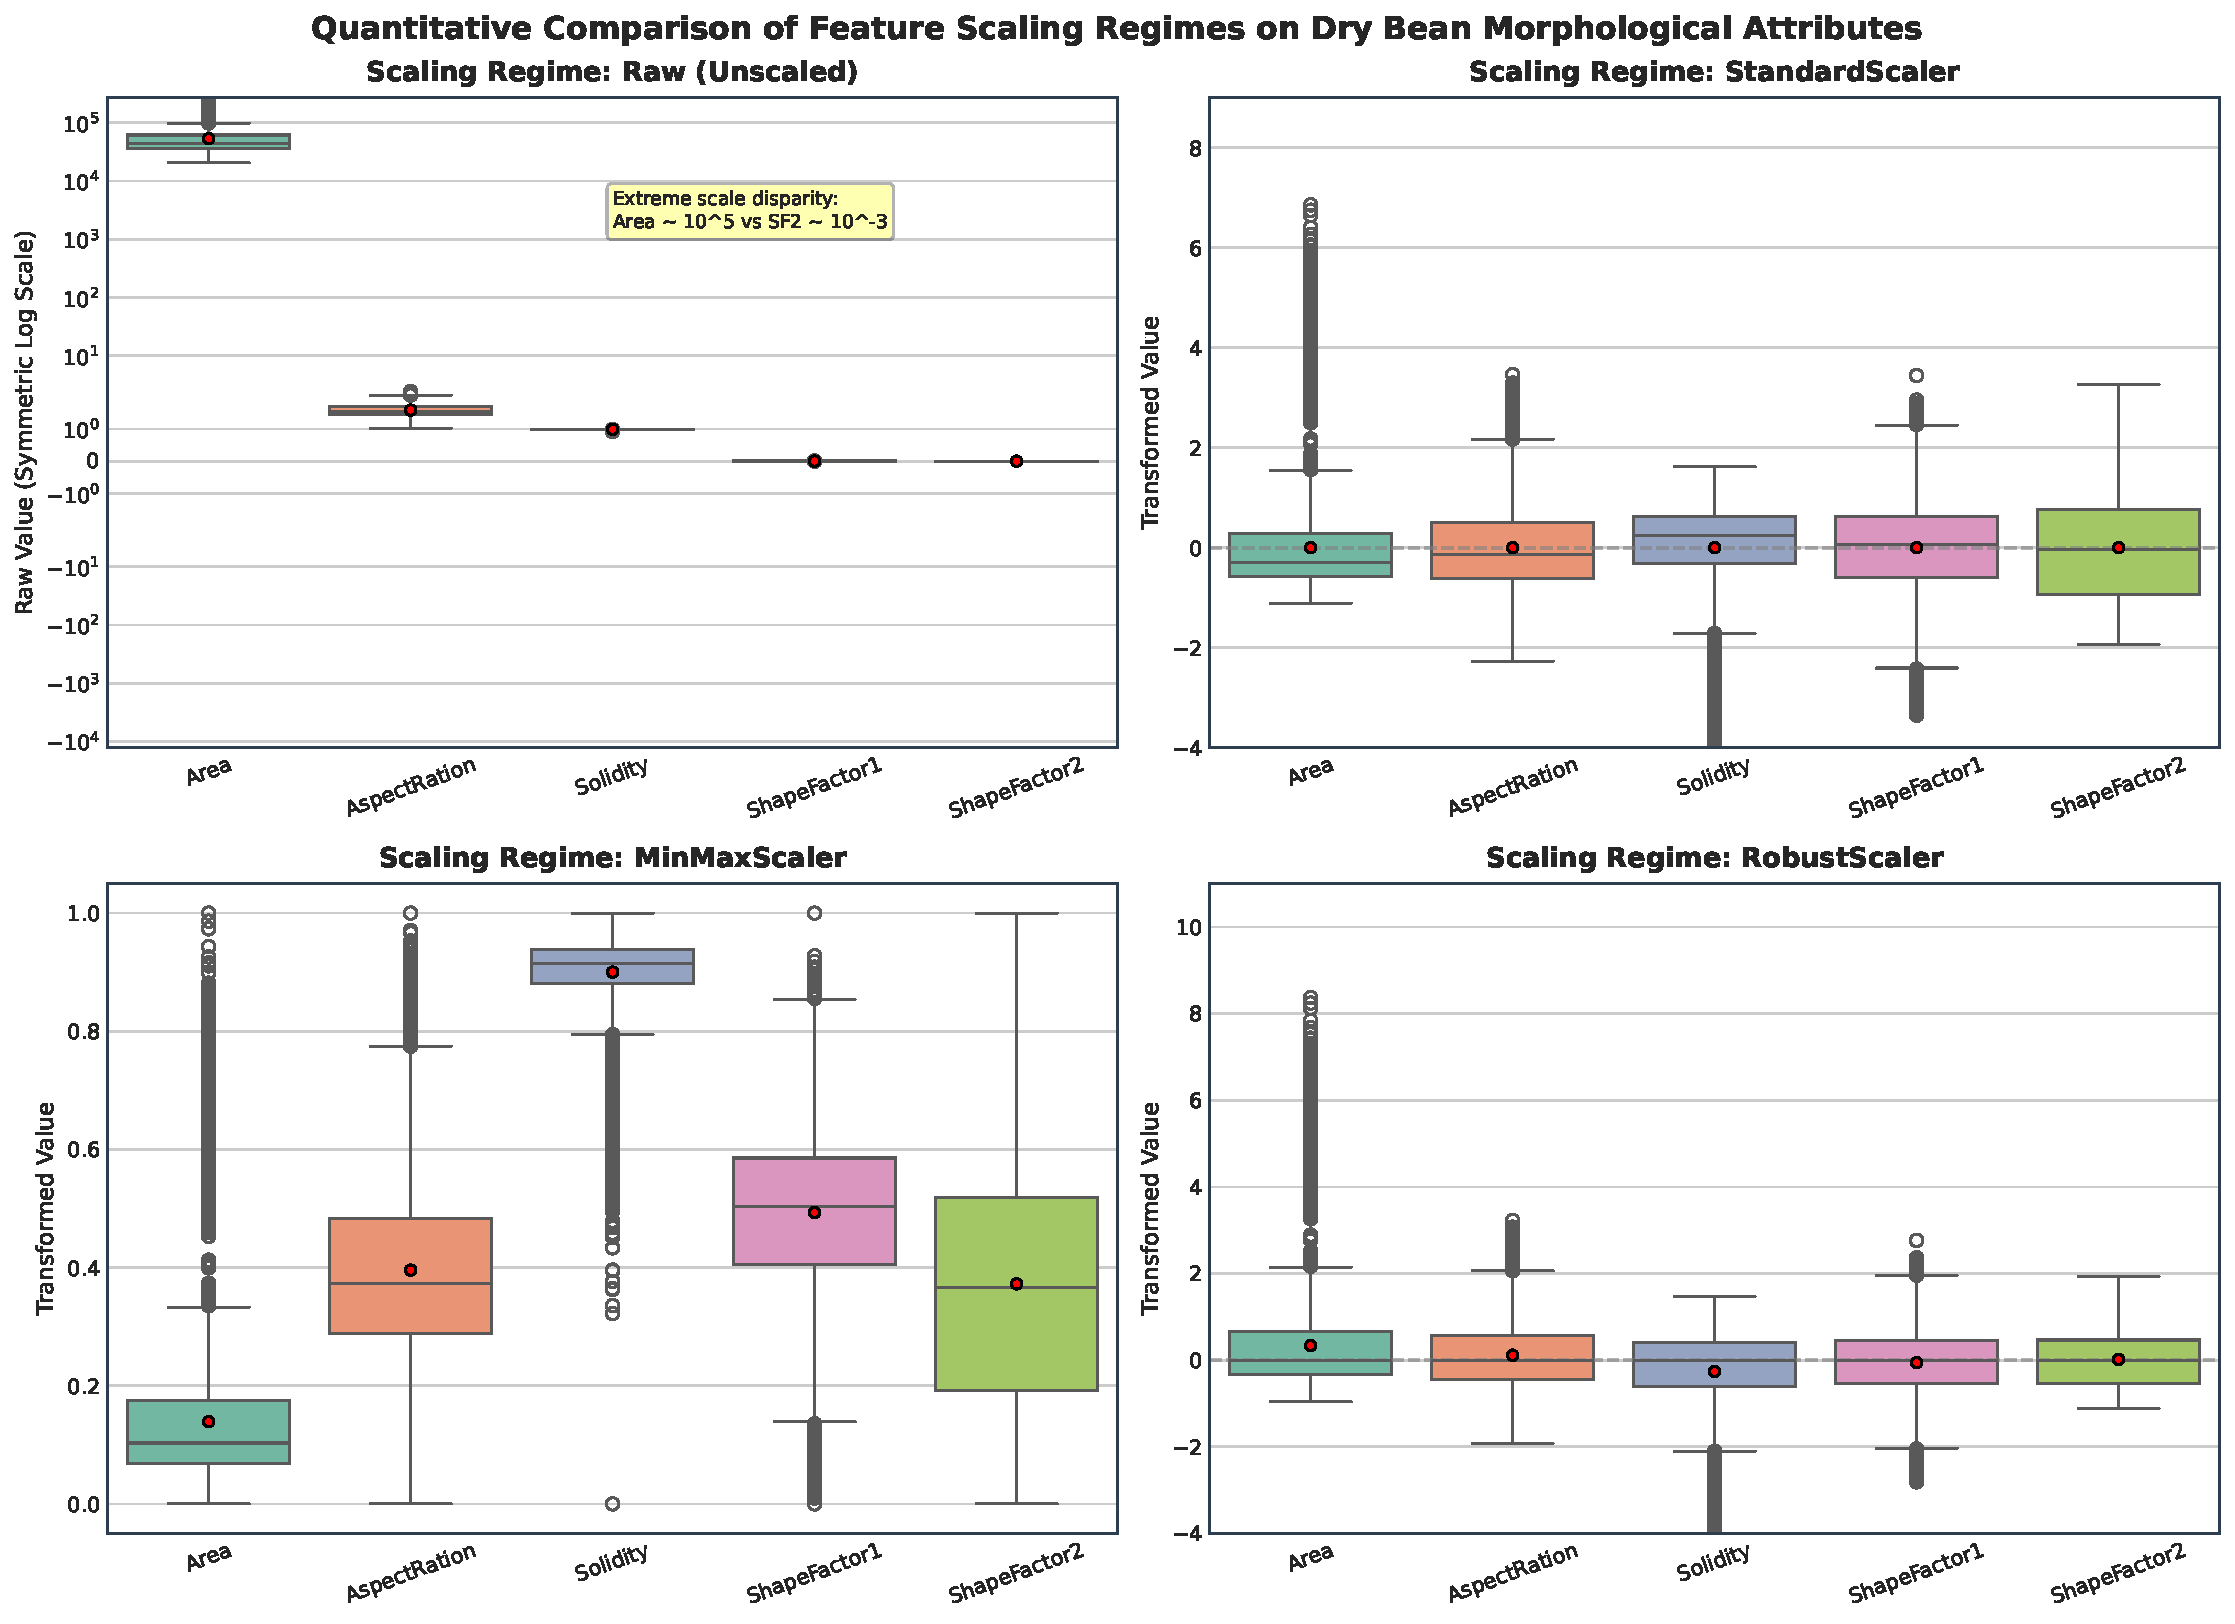
\includegraphics[width=0.88\linewidth]{fig01_scaling_comparison}
    \caption{Distributional distortion across feature scaling regimes: Unscaled Raw (extreme $75.5\text{M}\times$ disparity), StandardScaler (zero mean, unit variance), MinMaxScaler (bounded $[0, 1]$), and RobustScaler (median zero, IQR unit scale).}
    \label{fig:scaling_comp}
\end{figure}

\subsection{Multicollinearity Diagnostics and Feature Selection}
\label{subsec:multicollinearity}

We audit pairwise Pearson correlations across all 16 features. Exactly $21$ feature pairs exhibit $|r| \ge 0.90$, and $15$ pairs exceed $|r| \ge 0.95$. The correlation between \texttt{Area} and \texttt{ConvexArea} reaches $r = 0.9999$. Collinearity diagnostics via Variance Inflation Factors (VIF) reveal severe variance inflation:
\begin{equation}
    \text{VIF}_j = \frac{1}{1 - R_j^2}
\end{equation}
where $R_j^2$ is the coefficient of determination when regressing feature $j$ on all remaining predictive features. Table~\ref{tab:feature_selection} records VIFs and multi-criteria rankings via ANOVA $F$-values and Mutual Information (MI).

\begin{table}[htbp]
    \centering
    \small
    \caption{Multicollinearity Diagnostics (VIF), Feature Selection Ranking, and 8-Feature Pruned Subset.}
    \label{tab:feature_selection}
    \setlength{\tabcolsep}{5pt}
    \begin{tabularx}{\linewidth}{@{} l r r r c @{}}
        \toprule
        \textbf{Feature Name} & \textbf{VIF (16 Feat)} & \textbf{ANOVA $F$-Value} & \textbf{Mutual Info (MI)} & \textbf{Pruned 8 VIF} \\
        \midrule
        \texttt{EquivDiameter} & $317{,}671.59$ & $25{,}488.18$ & $1.0347$ & \textit{Pruned} \\
        \texttt{Compactness} & $275{,}722.88$ & $9{,}991.05$ & $0.8305$ & \textit{Pruned} \\
        \texttt{ShapeFactor3} & $199{,}791.01$ & $9{,}734.66$ & $0.8305$ & \textit{Pruned} \\
        \texttt{MajorAxisLength} & $88{,}521.08$ & $21{,}631.47$ & $0.9934$ & \textit{Pruned} \\
        \texttt{Area} & $81{,}784.07$ & $29{,}014.84$ & $1.0353$ & $5.05$ \\
        \texttt{ConvexArea} & $78{,}927.31$ & $28{,}960.45$ & $1.0380$ & \textit{Pruned} \\
        \texttt{MinorAxisLength} & $78{,}064.60$ & $22{,}431.93$ & $0.9275$ & \textit{Pruned} \\
        \texttt{AspectRation} & $13{,}800.55$ & $10{,}198.17$ & $0.8145$ & $17.67$ \\
        \texttt{Perimeter} & $3{,}576.33$ & $24{,}327.02$ & $1.0551$ & \textit{Pruned} \\
        \texttt{ShapeFactor2} & $1{,}242.07$ & $12{,}203.84$ & $0.9534$ & $\mathbf{18.44}$ \\
        \texttt{Eccentricity} & $1{,}180.05$ & $8{,}159.78$ & $0.8145$ & \textit{Pruned} \\
        \texttt{ShapeFactor1} & $608.60$ & $12{,}101.10$ & $0.9294$ & $8.30$ \\
        \texttt{roundness} & $103.30$ & $6{,}069.85$ & $0.7955$ & $7.04$ \\
        \texttt{ShapeFactor4} & $66.68$ & $1{,}263.08$ & $0.3630$ & $3.42$ \\
        \texttt{Solidity} & $14.02$ & $633.40$ & $0.2306$ & $4.71$ \\
        \texttt{Extent} & $1.24$ & $427.25$ & $0.1972$ & $1.23$ \\
        \bottomrule
    \end{tabularx}
\end{table}

By pruning redundant geometric duplicates, our selected 8-feature subset (\texttt{Area}, \texttt{AspectRation}, \texttt{Extent}, \texttt{Solidity}, \texttt{roundness}, \texttt{ShapeFactor1}, \texttt{ShapeFactor2}, \texttt{ShapeFactor4}) slashes the maximum VIF from $317{,}671.59$ to $18.44$, eliminating ill-conditioned matrix inversion. Figure~\ref{fig:corr_heatmap} presents the full $16\times 16$ Pearson correlation heatmap.

\begin{figure}[htbp]
    \centering
    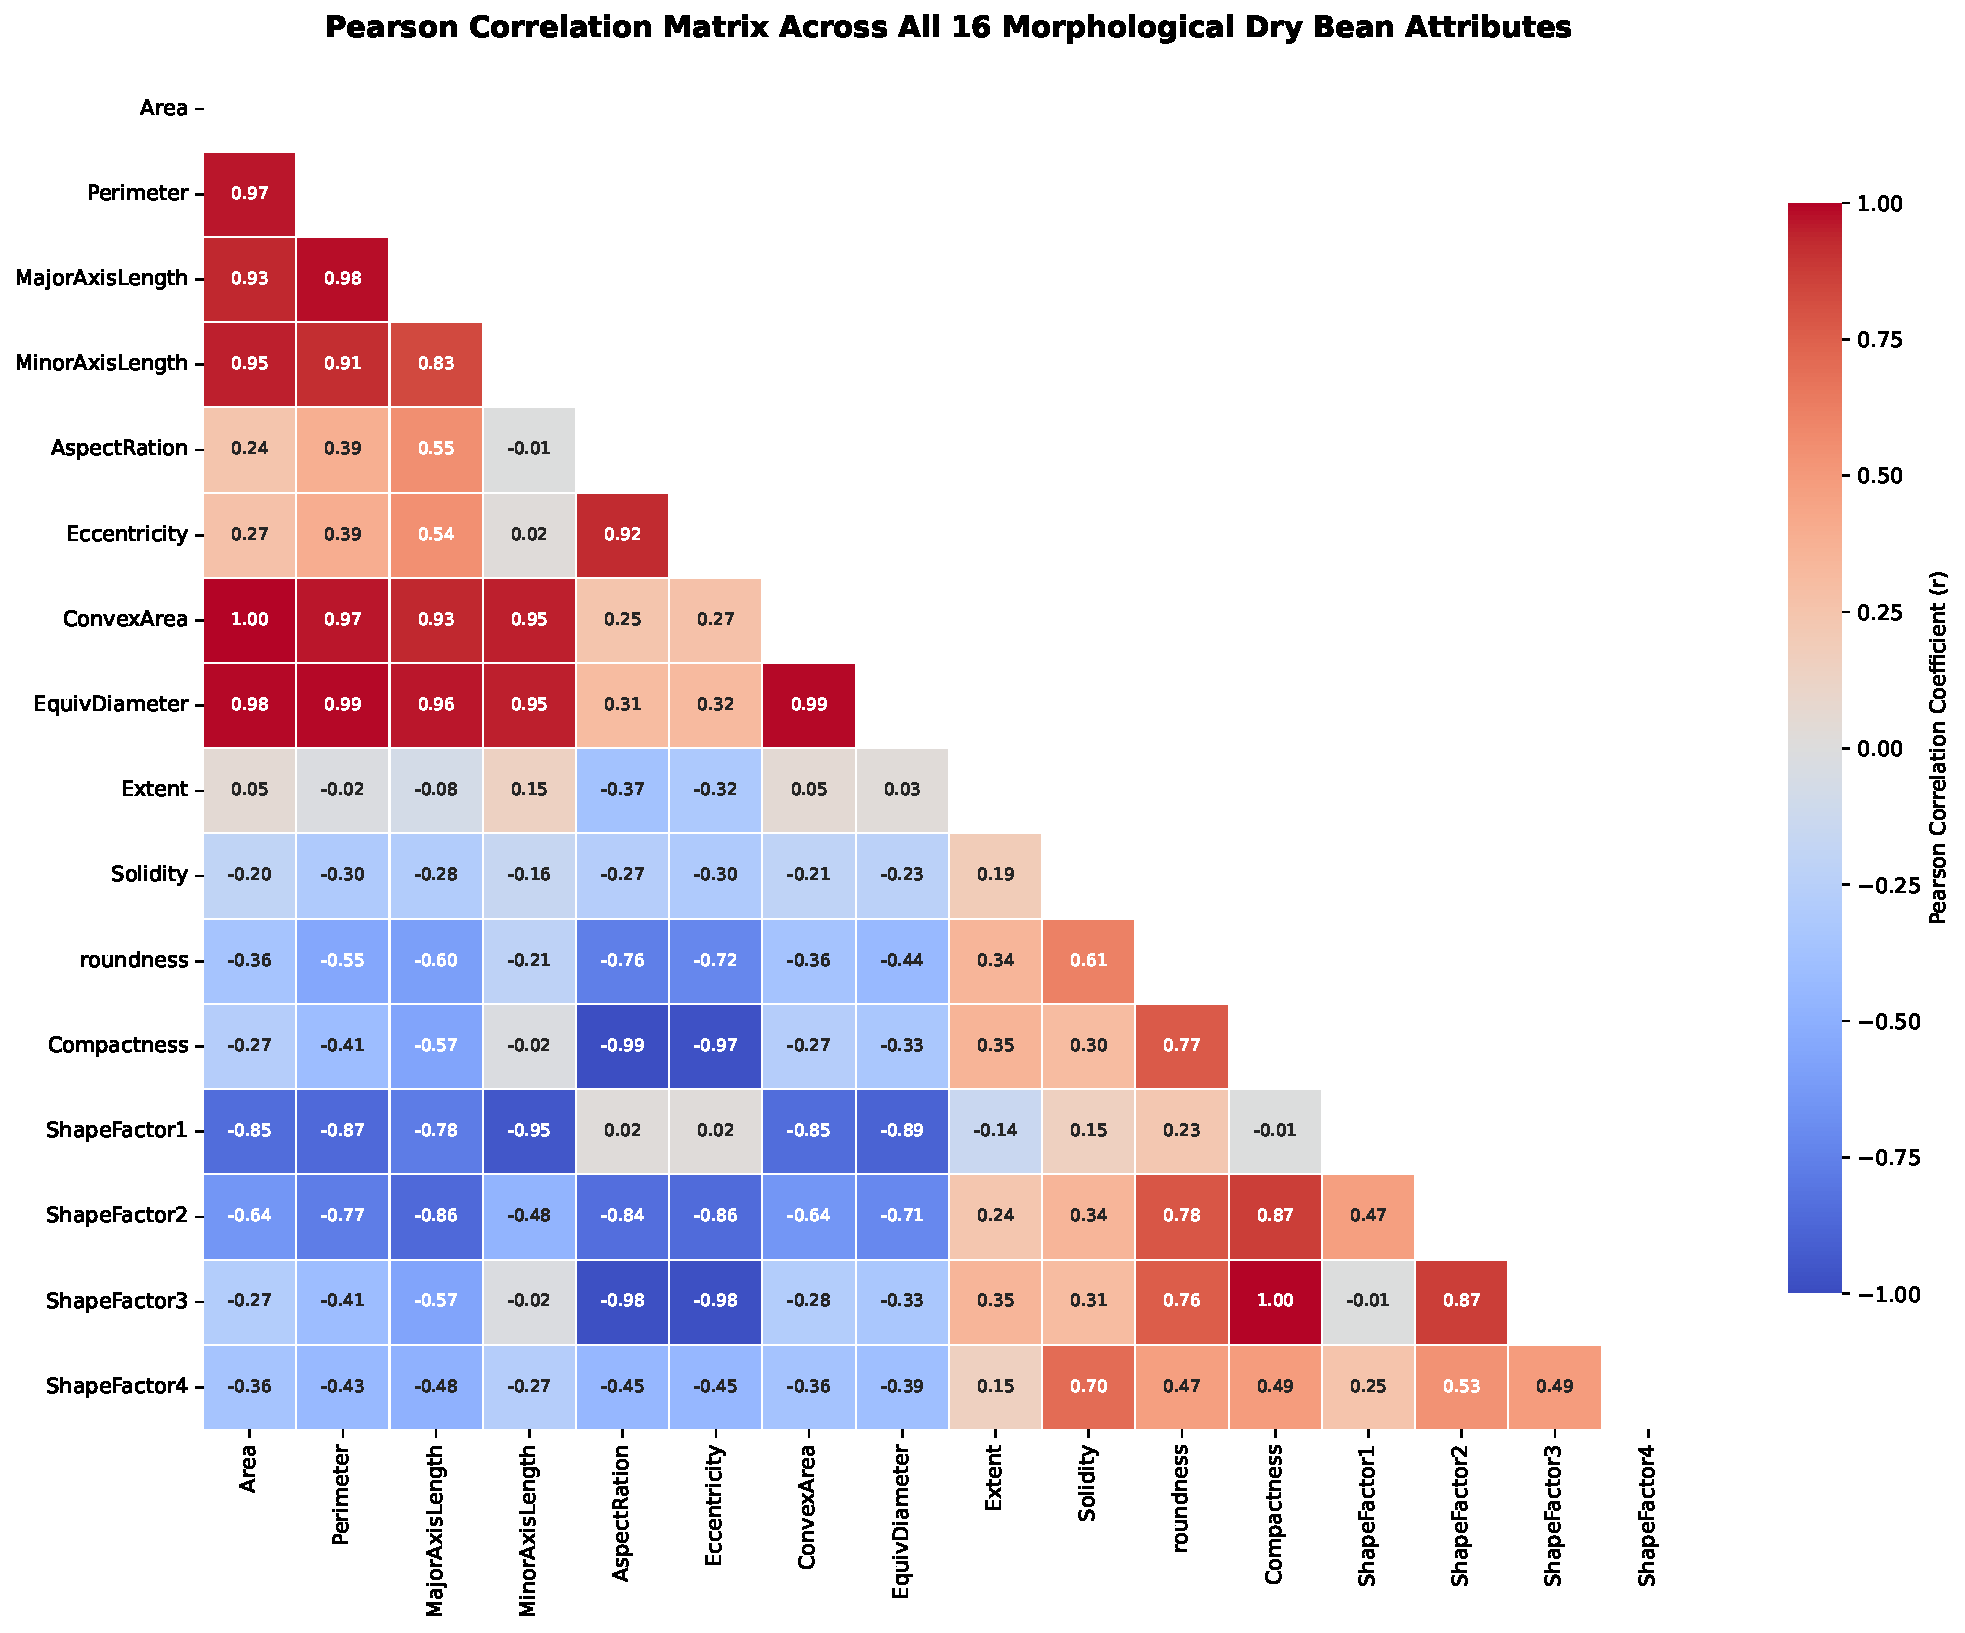
\includegraphics[width=0.88\linewidth]{fig06_correlation_heatmap}
    \caption{Pearson correlation matrix across all 16 morphological attributes, highlighting severe collinearity blocks among size features ($r \ge 0.98$) and shape factors.}
    \label{fig:corr_heatmap}
\end{figure}

\subsection{Principal Component Analysis (PCA)}
\label{subsec:pca}

We fit Principal Component Analysis on standardized features. PC1 explains $55.55\%$ of total variance, dominated by size metrics (\texttt{Area}, \texttt{Perimeter}, \texttt{EquivDiameter}). PC2 explains $26.36\%$, dominated by shape and elongation factors (\texttt{AspectRation}, \texttt{Compactness}, \texttt{roundness}). Cumulatively, PC1 and PC2 explain $81.91\%$ of all morphological variance, and $4$ components are required to reach the $95.00\%$ variance retention threshold. Figure~\ref{fig:pca_scree} depicts the PCA scree curve and 2D projection.

\begin{figure}[htbp]
    \centering
    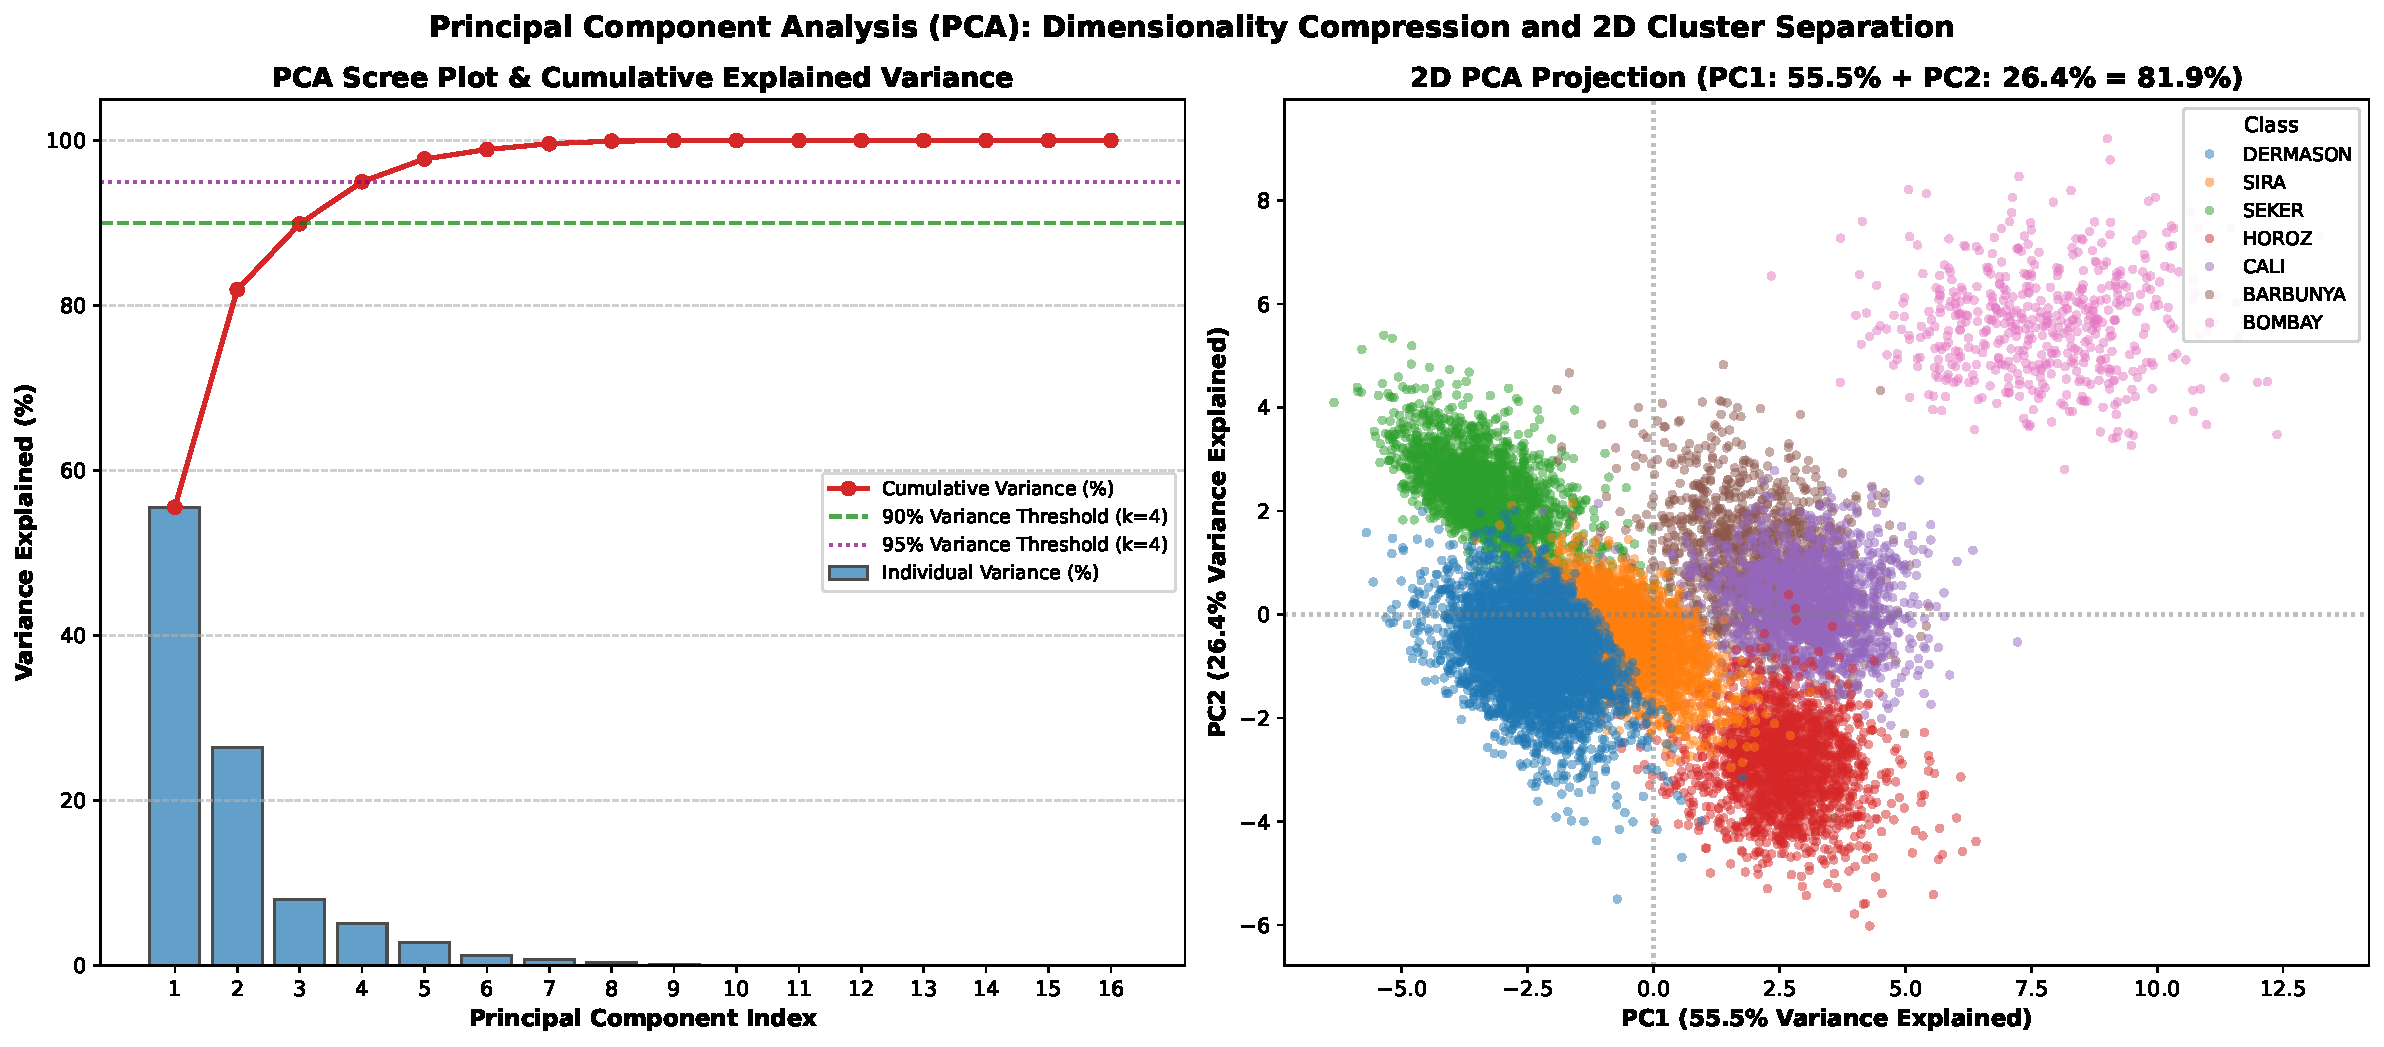
\includegraphics[width=0.88\linewidth]{fig07_pca_scree_and_projection}
    \caption{Principal Component Analysis (PCA): (Left) Scree plot and cumulative variance showing 4 PCs reach $95.00\%$ variance; (Right) 2D projection on PC1 (Size) and PC2 (Shape) colored by cultivar.}
    \label{fig:pca_scree}
\end{figure}

% ==============================================================================
% SECTION 4: EXPLORATORY DATA ANALYSIS
% ==============================================================================
\section{Exploratory Data Analysis}
\label{sec:eda}

Exploratory analysis reveals that dry bean varieties occupy structured clusters governed by two physical dimensions: grain volume and cross-sectional elongation.

\subsection{Univariate Distributions and Skewness}
\label{subsec:univariate_eda}

Size attributes (\texttt{Area}, \texttt{Perimeter}, \texttt{MajorAxisLength}) display substantial positive skewness ($> 1.25$) due to the long right tail introduced by the giant \texttt{BOMBAY} cultivar. Conversely, derived bounding metrics such as \texttt{Solidity} and \texttt{ShapeFactor4} exhibit extreme leptokurtic concentration near unity ($S \approx 0.985$--$0.995$), reflecting smooth convex grain contours. Figure~\ref{fig:feat_dist} illustrates the density distributions across six representative morphological features (\texttt{Area}, \texttt{Perimeter}, \texttt{MajorAxisLength}, \texttt{AspectRation}, \texttt{Solidity}, and \texttt{ShapeFactor1}).

\begin{figure}[htbp]
    \centering
    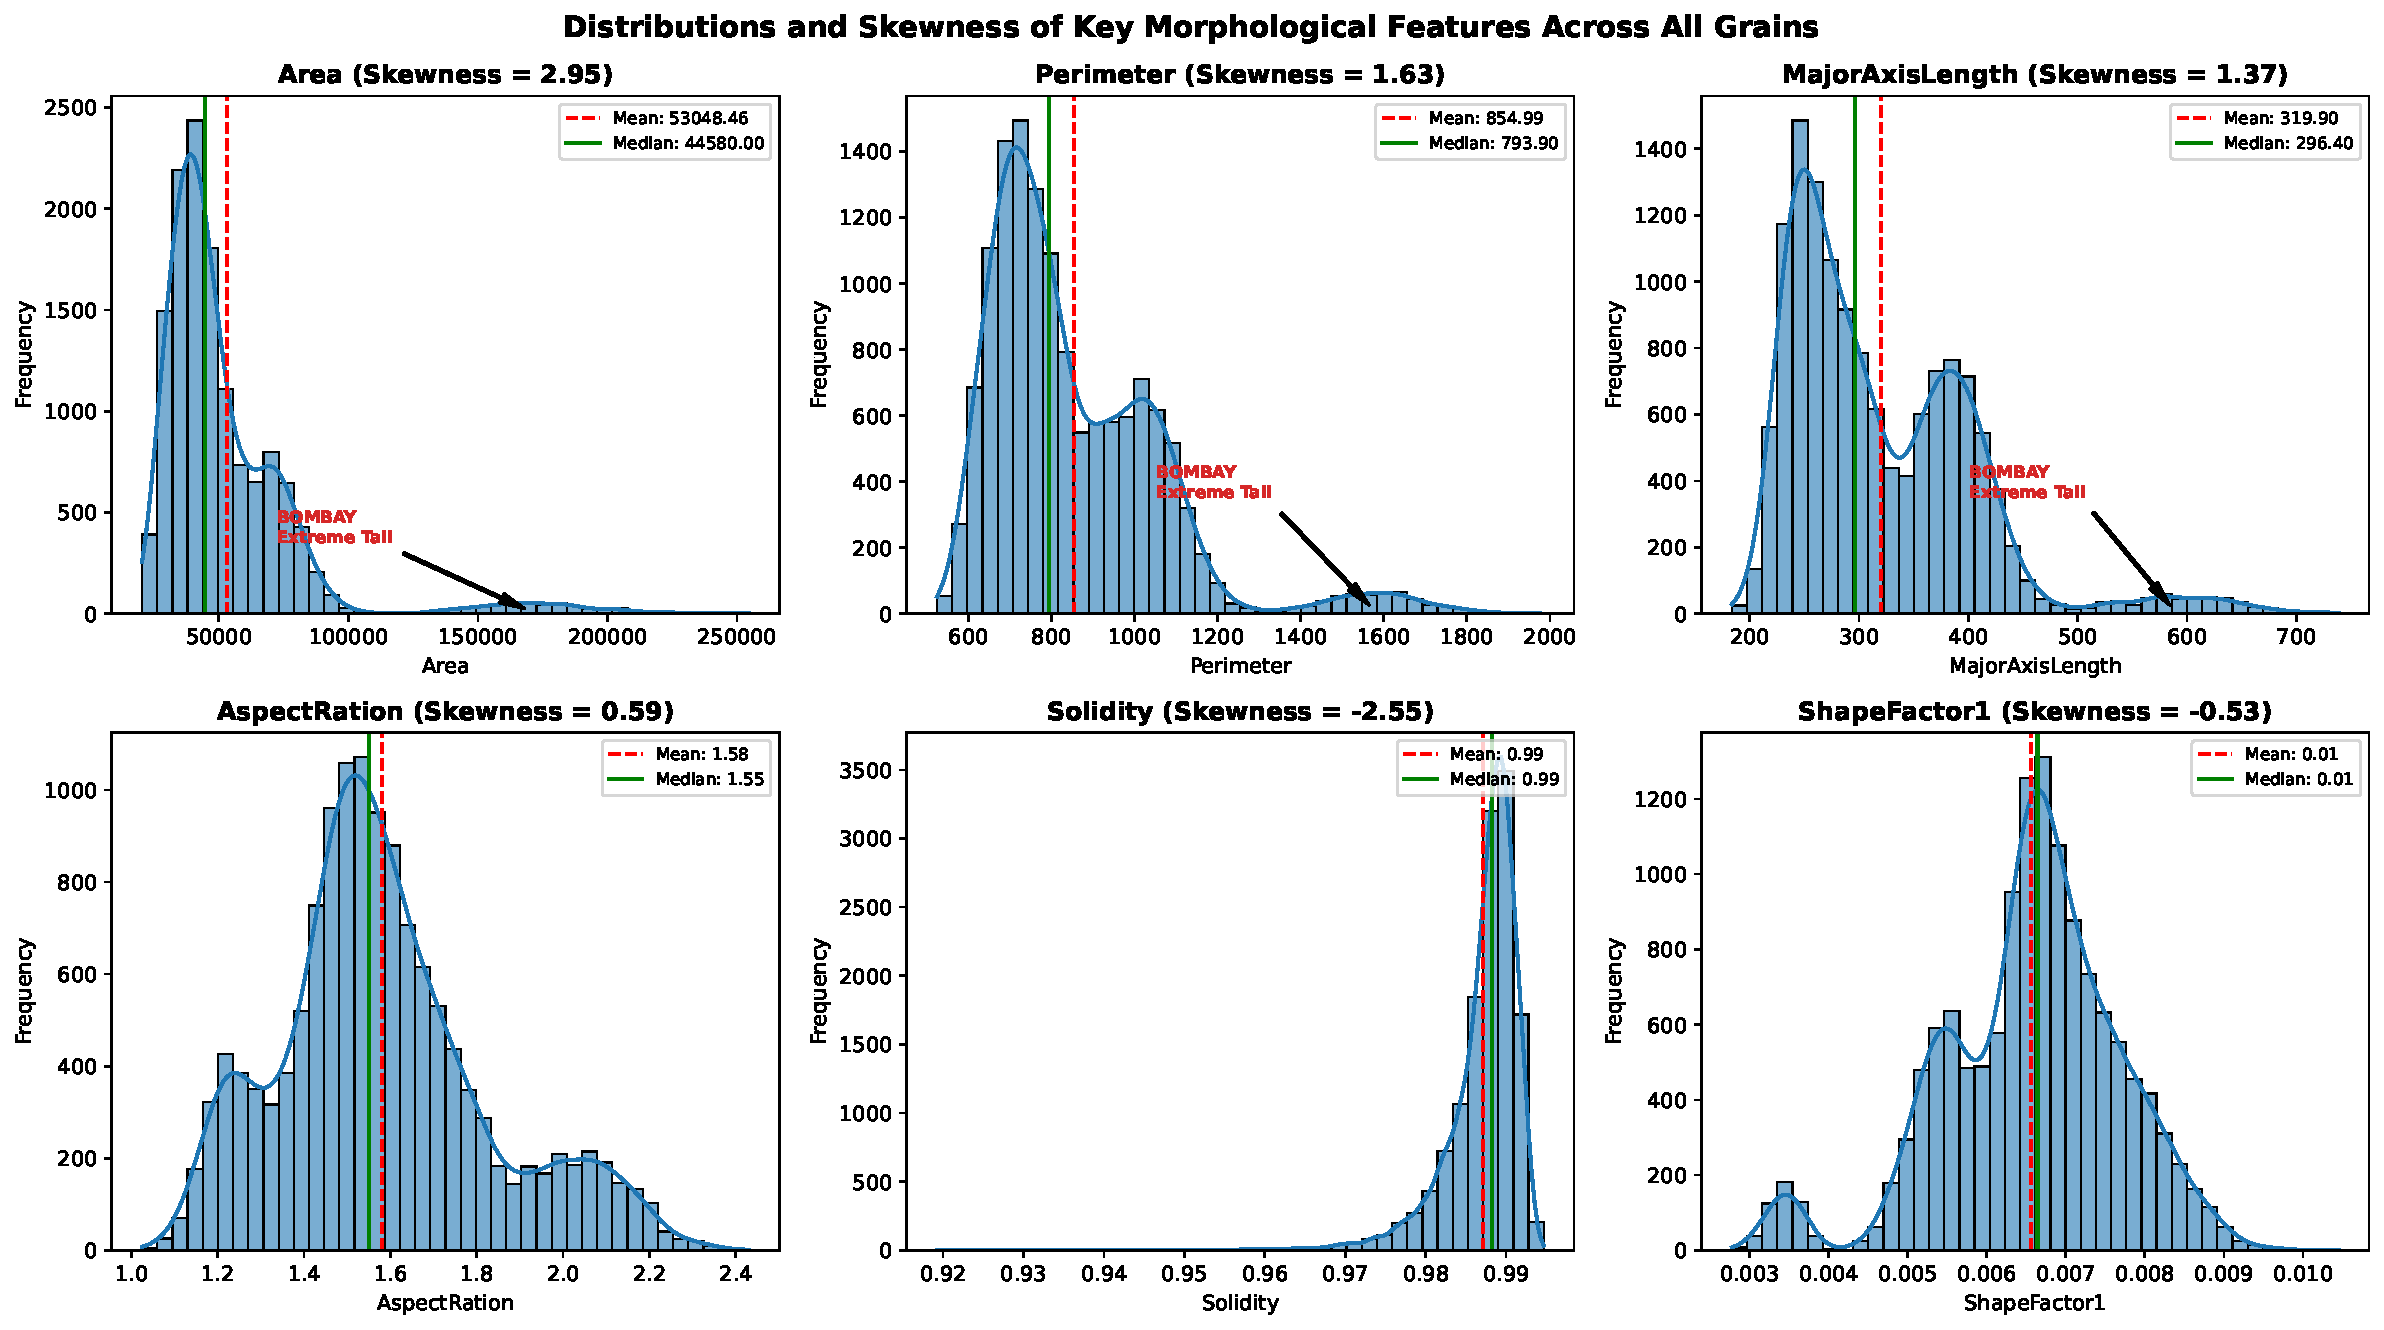
\includegraphics[width=0.92\linewidth]{fig03_feature_distributions}
    \caption{Kernel density estimates (KDE) and histograms across six representative morphological features (\texttt{Area}, \texttt{Perimeter}, \texttt{MajorAxisLength}, \texttt{AspectRation}, \texttt{Solidity}, and \texttt{ShapeFactor1}) for the deduplicated dataset ($N = 13{,}543$).}
    \label{fig:feat_dist}
\end{figure}

\subsection{Cultivar Stratified Boxplots and Bivariate Relationships}
\label{subsec:bivariate_eda}

Figure~\ref{fig:outlier_boxplots} contrasts global outlier distributions against cultivar-stratified boxplots. Within its own subpopulation, \texttt{BOMBAY} exhibits a standard Gaussian-like distribution with minimal intra-class outliers, reinforcing our decision to reject global outlier filtering.

\begin{figure}[htbp]
    \centering
    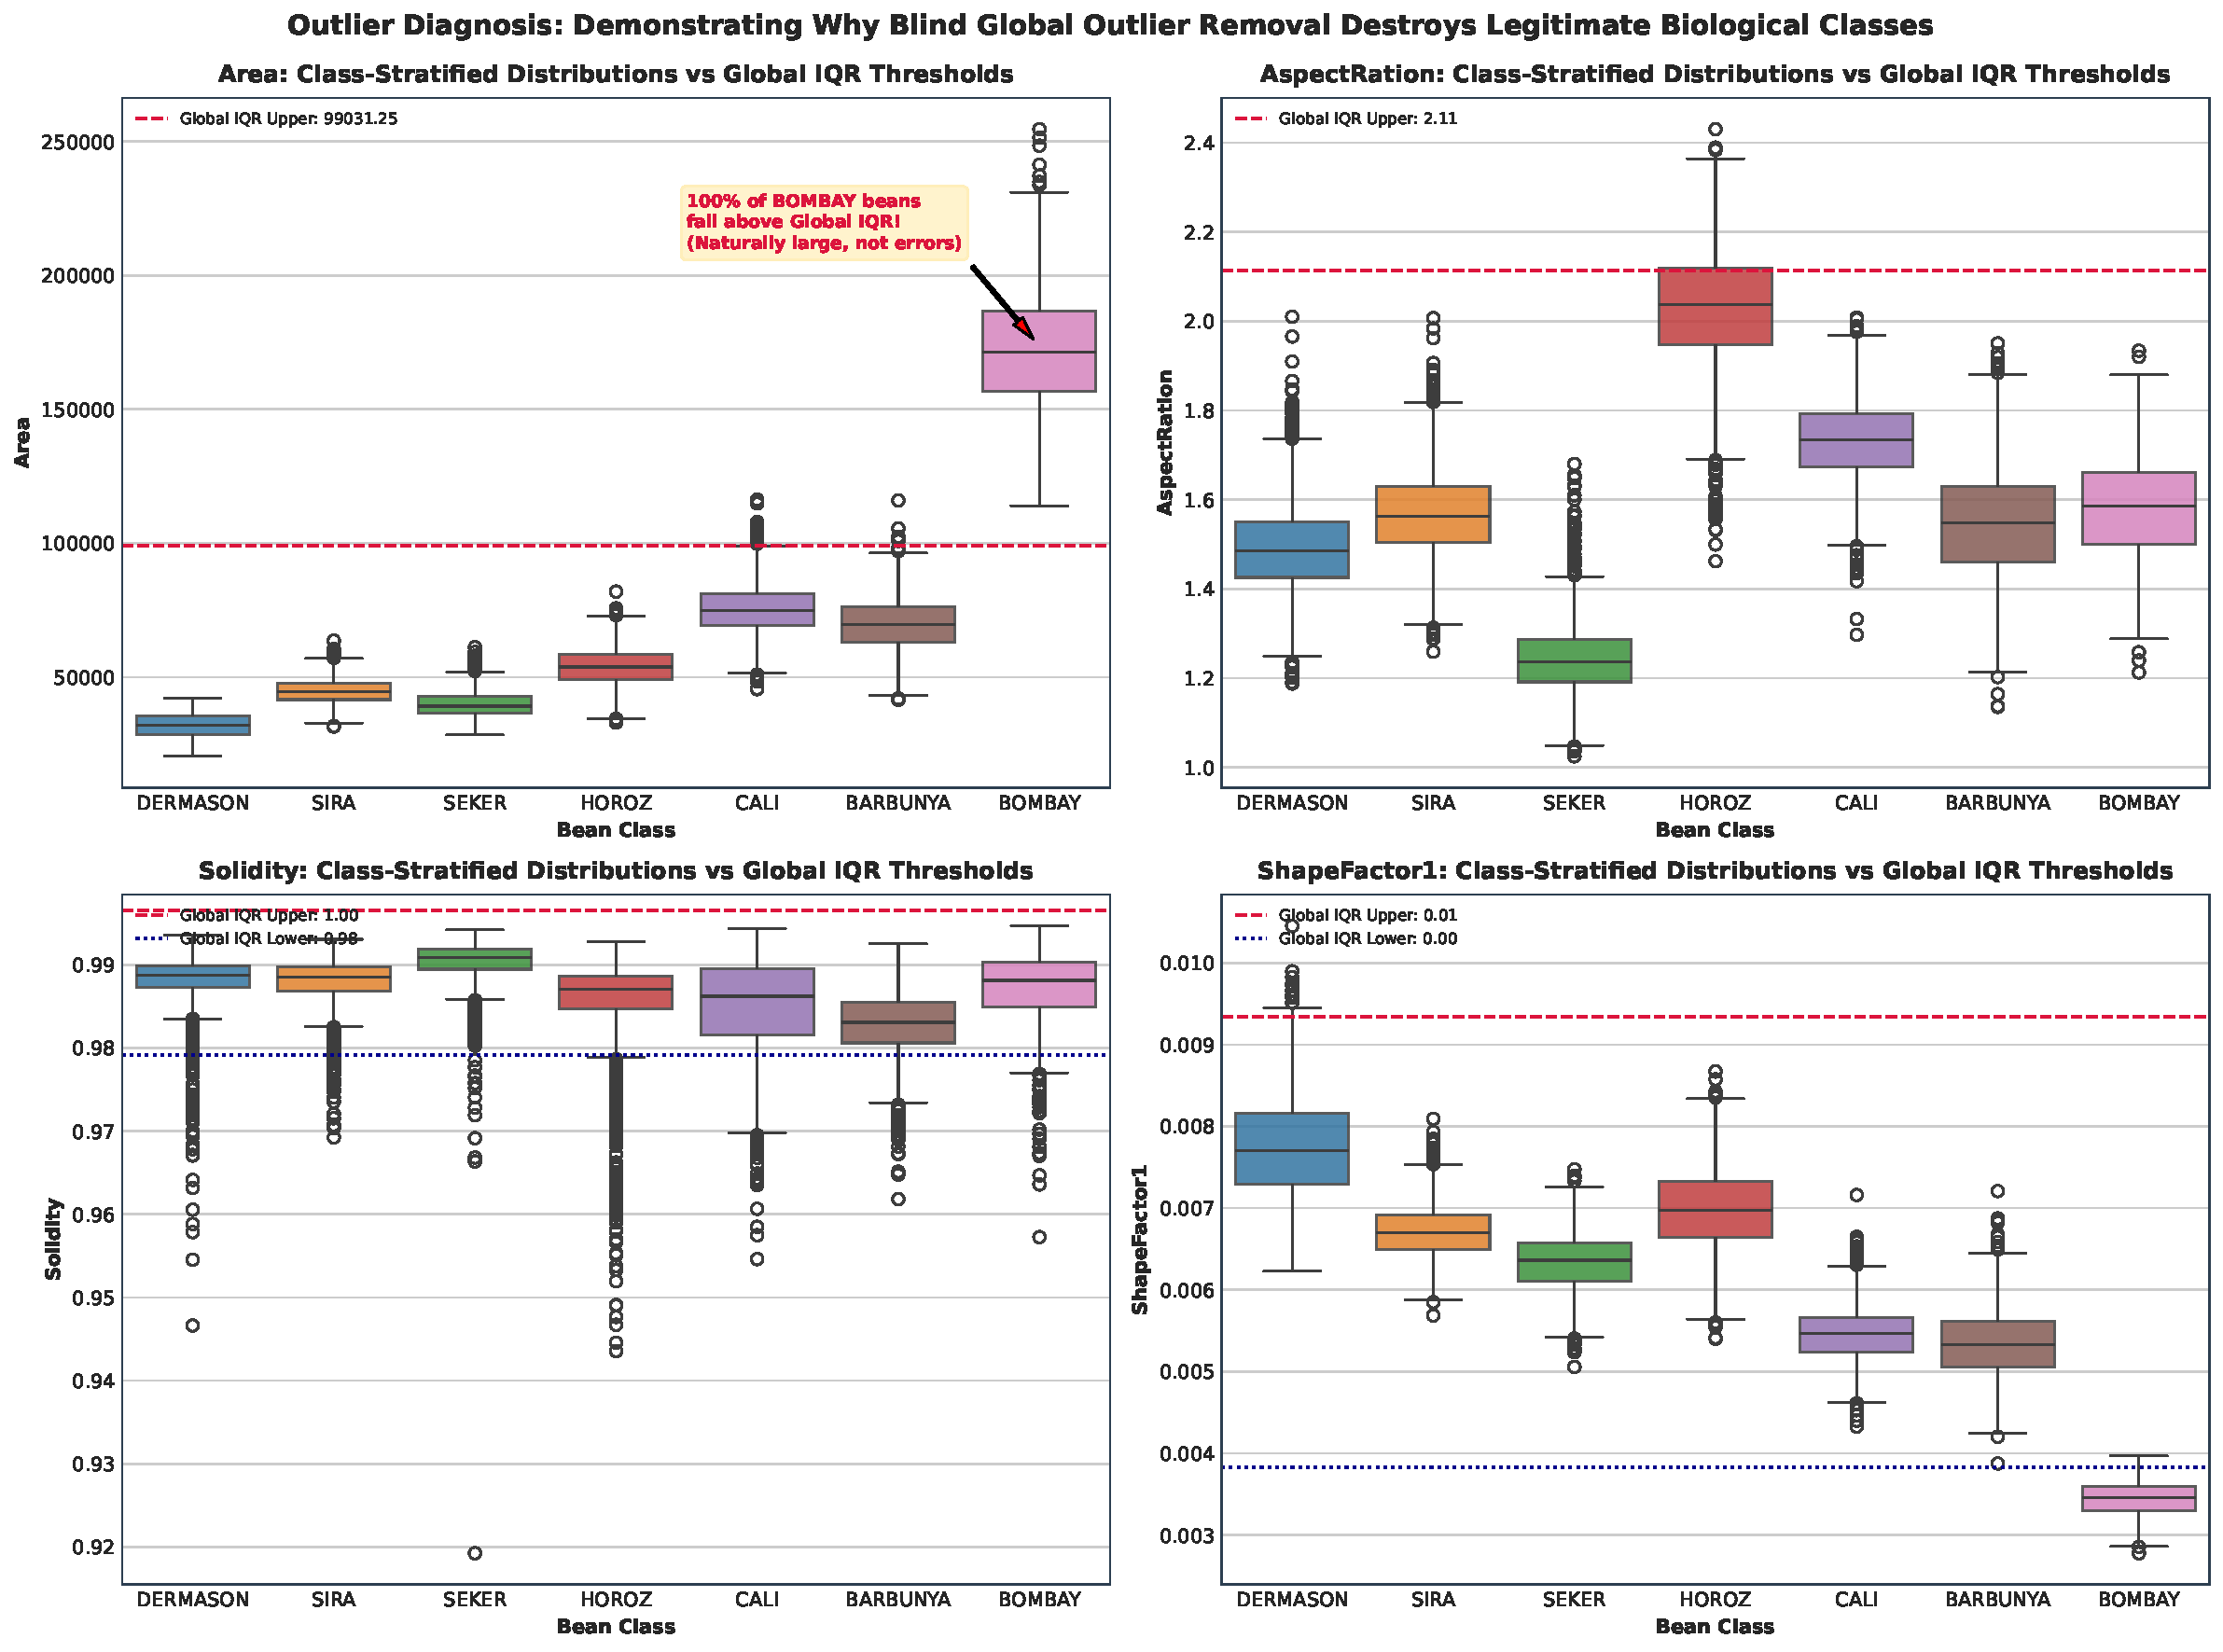
\includegraphics[width=0.88\linewidth]{fig04_outlier_boxplots_by_class}
    \caption{Cultivar-stratified boxplots for \texttt{Area}, \texttt{AspectRation}, \texttt{Solidity}, and \texttt{ShapeFactor1}, demonstrating clear separation of \texttt{BOMBAY} and overlapping profiles between \texttt{SIRA} and \texttt{DERMASON}.}
    \label{fig:outlier_boxplots}
\end{figure}

Bivariate scatter plots in Figure~\ref{fig:scatter_rel} reveal clear morphological archetypes:
\begin{itemize}[leftmargin=1.5em]
    \item \texttt{BOMBAY} forms an entirely isolated island in the high-Area, moderate-AspectRatio quadrant ($A > 114{,}000$).
    \item \texttt{SEKER} separates cleanly by high circularity ($R > 0.85$) and low AspectRatio ($K < 1.35$).
    \item \texttt{HOROZ} occupies the high AspectRatio ($K > 1.8$), low roundness ($R < 0.70$) regime.
    \item \texttt{DERMASON} and \texttt{SIRA} heavily overlap in the small Area, moderate AspectRatio quadrant, creating the primary decision boundary challenge.
    \item \texttt{BARBUNYA} and \texttt{CALI} overlap in the medium-large size regime, separated primarily by \texttt{roundness} and \texttt{Solidity}.
\end{itemize}

\begin{figure}[htbp]
    \centering
    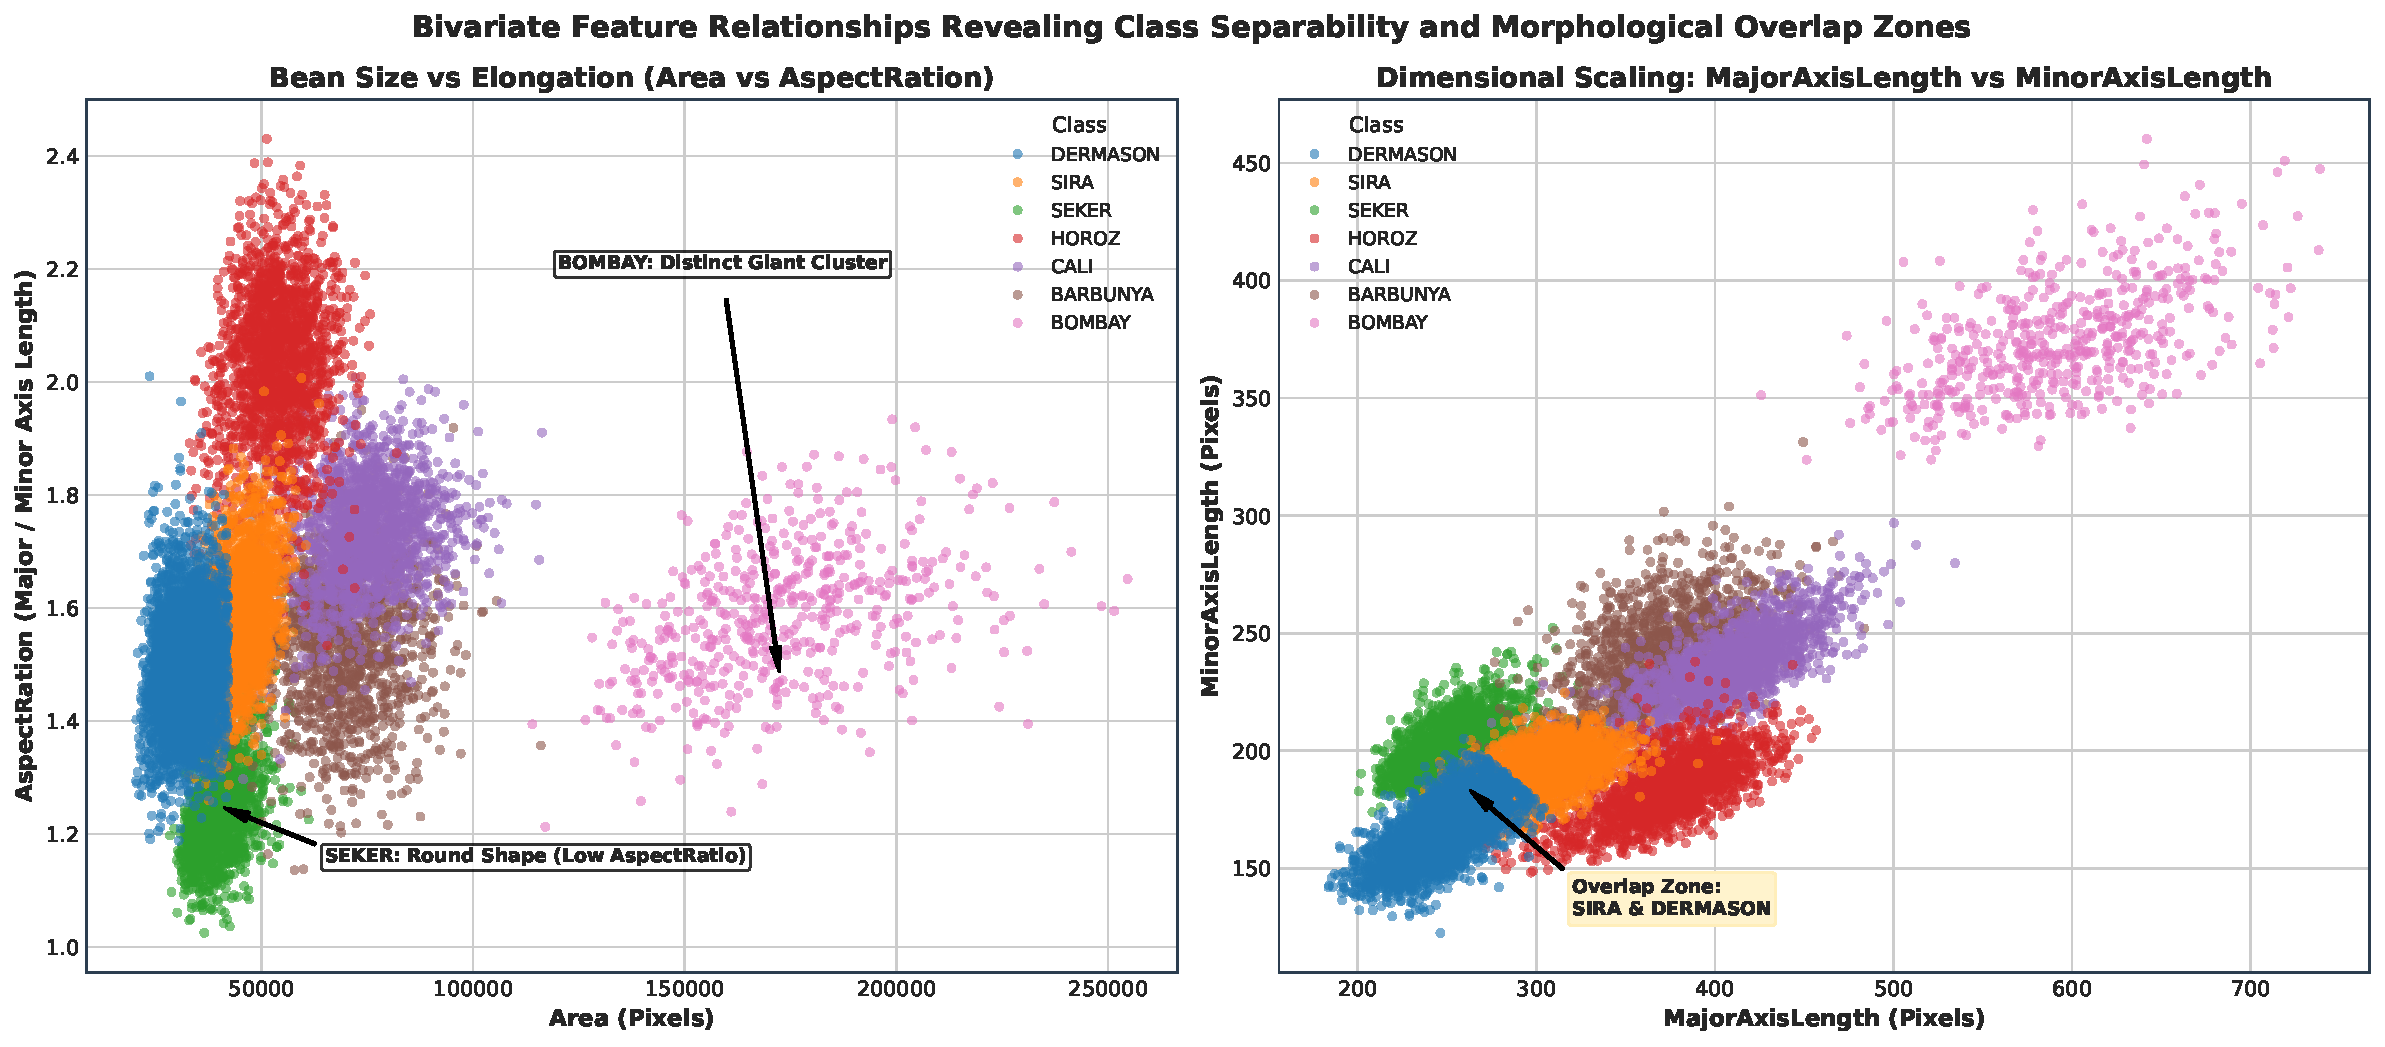
\includegraphics[width=0.88\linewidth]{fig05_relationship_scatter}
    \caption{Pairwise morphological relationships: (Left) Bean Size vs. Elongation (\texttt{Area} vs. \texttt{AspectRation}) and (Right) Dimensional Scaling (\texttt{MajorAxisLength} vs. \texttt{MinorAxisLength}), mapping cultivar separability.}
    \label{fig:scatter_rel}
\end{figure}

% ==============================================================================
% SECTION 5: METHODOLOGY
% ==============================================================================
\section{Methodology}
\label{sec:methodology}

We implement standard, mathematically principled data mining techniques across four paradigms using Python scientific packages~\citep{mckinney2010data,harris2020array,hunter2007matplotlib,waskom2021seaborn,pedregosa2011scikit,raschka2018mlxtend}:

\subsection{Similarity and Distance Metrics}
\label{subsec:meth_similarity}

We evaluate distance metrics on $d$-dimensional normalized feature vectors $\mathbf{u}, \mathbf{v} \in \mathbb{R}^d$:
\begin{align}
    \text{Euclidean } (L_2): \quad & d_2(\mathbf{u}, \mathbf{v}) = \sqrt{\sum_{i=1}^d (u_i - v_i)^2} \\
    \text{Manhattan } (L_1): \quad & d_1(\mathbf{u}, \mathbf{v}) = \sum_{i=1}^d |u_i - v_i| \\
    \text{Cosine Distance}: \quad & d_{\cos}(\mathbf{u}, \mathbf{v}) = 1 - \frac{\mathbf{u} \cdot \mathbf{v}}{\|\mathbf{u}\|_2 \|\mathbf{v}\|_2}
\end{align}
For unit-normalized vectors ($\|\mathbf{u}\|_2 = \|\mathbf{v}\|_2 = 1$), Cosine distance is strictly monotonic with squared Euclidean distance: $d_2^2(\mathbf{u}, \mathbf{v}) = 2 d_{\cos}(\mathbf{u}, \mathbf{v})$, allowing efficient exact nearest-neighbor indexing.

Nearest-neighbor concordance is evaluated via Jaccard overlap on top-$k$ neighbor index sets $\mathcal{N}_A(\mathbf{x}_i)$ and $\mathcal{N}_B(\mathbf{x}_i)$:
\begin{equation}
    J_k(\mathbf{x}_i) = \frac{|\mathcal{N}_A(\mathbf{x}_i) \cap \mathcal{N}_B(\mathbf{x}_i)|}{|\mathcal{N}_A(\mathbf{x}_i) \cup \mathcal{N}_B(\mathbf{x}_i)|}
\end{equation}
Neighbor class purity is computed as the fraction of top-$k$ neighbors sharing the target bean's true cultivar label:
\begin{equation}
    \text{Purity}_k(\mathbf{x}_i) = \frac{1}{k} \sum_{\mathbf{x}_j \in \mathcal{N}(\mathbf{x}_i)} \mathbb{I}(y_j = y_i)
\end{equation}

\subsection{Unsupervised Clustering Algorithms}
\label{subsec:meth_clustering}

We evaluate three foundational clustering algorithms (excluding \texttt{Class} labels during fitting):
\begin{enumerate}[leftmargin=1.5em]
    \item \textbf{$k$-Means Clustering~\citep{lloyd1982least}:} Minimizes Within-Cluster Sum of Squares (WCSS / Inertia):
    \begin{equation}
        \mathcal{J}_{k\text{-Means}} = \sum_{k=1}^K \sum_{\mathbf{x}_i \in \mathcal{C}_k} \|\mathbf{x}_i - \boldsymbol{\mu}_k\|_2^2
    \end{equation}
    where $\boldsymbol{\mu}_k$ is the empirical centroid of cluster $\mathcal{C}_k$. Initialized with $k$-Means++ across $k \in [2, 10]$ with $10$ restarts.
    \item \textbf{Agglomerative Hierarchical Clustering~\citep{ward1963hierarchical}:} Employs Ward's minimum variance criterion, merging clusters $A$ and $B$ that minimize objective increase:
    \begin{equation}
        \Delta \text{ESS}_{AB} = \frac{n_A n_B}{n_A + n_B} \|\boldsymbol{\mu}_A - \boldsymbol{\mu}_B\|_2^2
    \end{equation}
    To prevent quadratic memory scaling ($O(N^2) \approx 1.5\text{ GB}$), Ward linkage is executed on a deterministic stratified subsample ($n = 2{,}500$, preserving exact cultivar proportions).
    \item \textbf{DBSCAN Density-Based Clustering~\citep{ester1996density}:} Groups core points possessing at least $\text{min\_samples}$ neighbors within distance $\varepsilon$:
    \begin{equation}
        \mathcal{N}_\varepsilon(\mathbf{x}) = \{\mathbf{x}' \in \mathcal{D} \mid d_2(\mathbf{x}, \mathbf{x}') \le \varepsilon\}
    \end{equation}
    Points failing density reachability are assigned to the unassigned noise cluster ($-1$).
\end{enumerate}

Cluster validation combines internal metrics (Silhouette score $s(i) = \frac{b(i) - a(i)}{\max(a(i), b(i))}$~\citep{rousseeuw1987silhouettes}, Calinski-Harabasz, Davies-Bouldin) and external agreement against ground truth cultivars via the Adjusted Rand Index (ARI)~\citep{hubert1985comparing} and Normalized Mutual Information (NMI).

\subsection{Supervised Classification Models}
\label{subsec:meth_classification}

We train four supervised classifiers on the stratified 80/20 train/test split ($N_{\text{train}} = 10{,}834$, $N_{\text{test}} = 2{,}709$), with all scalers fit strictly on training splits to prevent data leakage:
\begin{enumerate}[leftmargin=1.5em]
    \item \textbf{Decision Tree Classifier~\citep{breiman1984cart}:} Recursive binary partitioning optimizing Gini impurity:
    \begin{equation}
        I_G(t) = 1 - \sum_{c=1}^C p(c|t)^2
    \end{equation}
    Hyperparameters are tuned via 5-fold Stratified Cross-Validation on the training split, selecting \texttt{max\_depth=10} and \texttt{min\_samples\_leaf=5}.
    \item \textbf{Interpretable Rule-Based Classifier:} A constrained shallow decision tree (\texttt{max\_depth=4}) generating human-auditable IF-THEN rules with explicit rule coverage and precision.
    \item \textbf{Gaussian Naïve Bayes:} Maximum a posteriori classification assuming class-conditional feature independence:
    \begin{equation}
        P(y = c \mid \mathbf{x}) \propto P(y = c) \prod_{j=1}^d \frac{1}{\sqrt{2\pi\sigma_{cj}^2}} \exp\left(-\frac{(x_j - \mu_{cj})^2}{2\sigma_{cj}^2}\right)
    \end{equation}
    \item \textbf{$k$-Nearest Neighbors ($k$-NN)~\citep{cover1967nearest}:} Non-parametric majority voting among the $k = 7$ nearest Euclidean neighbors in standardized feature space.
\end{enumerate}

\subsection{Morphological Association Rule Mining}
\label{subsec:meth_association}

To discover interpretable morphological co-occurrence patterns without producing trivial geometric tautologies, we discretize five low-collinearity features (\texttt{Area}, \texttt{AspectRation}, \texttt{roundness}, \texttt{Solidity}, \texttt{Extent}) into tertiles (\texttt{Low}, \texttt{Medium}, \texttt{High}). Using the FP-Growth algorithm~\citep{han2000mining,raschka2018mlxtend}, we extract frequent itemsets at minimum support $\text{minsup} = 0.02$ and mine Class Association Rules (CARs) where consequents are constrained to a single cultivar label ($\mathcal{A} \to \{Class = c\}$):
\begin{align}
    \text{Support}(\mathcal{A} \to \mathcal{B}) &= P(\mathcal{A} \cup \mathcal{B}) \\
    \text{Confidence}(\mathcal{A} \to \mathcal{B}) &= \frac{P(\mathcal{A} \cup \mathcal{B})}{P(\mathcal{A})} \\
    \text{Lift}(\mathcal{A} \to \mathcal{B}) &= \frac{P(\mathcal{A} \cup \mathcal{B})}{P(\mathcal{A}) P(\mathcal{B})}
\end{align}

\subsection{The Group 10 Data Mining Stress-Test Protocol}
\label{subsec:meth_stress_protocol}

The core experimental contribution subjects the clean baseline pipeline to four controlled degradation axes:
\begin{enumerate}[leftmargin=1.5em]
    \item \textbf{Stress Test 1 (Missing Data MCAR):} Missing Completely at Random values are injected at $0\%, 5\%, 10\%, 20\%, 30\%$ across predictive features. We compare Median Imputation against $k$-NN Imputation ($k = 5$), fit strictly on corrupted training splits.
    \item \textbf{Stress Test 2 (Outlier Injection):} Sensor/segmentation glitches are simulated by injecting $+8\sigma$ spikes into $0\%, 5\%, 10\%, 20\%$ of training records across randomly selected features.
    \item \textbf{Stress Test 3 (Normalization Sensitivity):} We benchmark Raw, StandardScaler, MinMaxScaler, and RobustScaler under both Clean ($0\%$ outliers) and Corrupted ($10\%$ outliers) regimes.
    \item \textbf{Stress Test 4 (Dimensionality and Collinearity):} We contrast all 16 features (max VIF $= 317{,}671.59$), the pruned 8-feature subset (max VIF $= 18.44$), PCA with 4 components ($95.00\%$ variance), and PCA with 2 components ($81.91\%$ variance).
\end{enumerate}

% ==============================================================================
% SECTION 6: EXPERIMENTAL RESULTS
% ==============================================================================
\section{Experimental Results}
\label{sec:results}

\subsection{Similarity and Distance Metric Analysis}
\label{subsec:res_similarity}

Table~\ref{tab:similarity} records the empirical concordance across distance metrics and scaling transformations, visualized in Figure~\ref{fig:dist_comp}.

\begin{table}[htbp]
    \centering
    \small
    \caption{Empirical Nearest-Neighbor Concordance ($k=10$) Across Distance Metrics and Scalers.}
    \label{tab:similarity}
    \setlength{\tabcolsep}{4.5pt}
    \begin{tabularx}{\linewidth}{@{} l >{\raggedright\arraybackslash}X cccc @{}}
        \toprule
        \textbf{Type} & \textbf{Comparison (A vs. B)} & \textbf{Jaccard @10} & \textbf{1-NN Agree} & \textbf{Purity A} & \textbf{Purity B} \\
        \midrule
        \multirow{3}{*}{\textbf{Metric}} & $L_2$ (Std) vs. $L_1$ (Std) & $0.4676$ & $0.5212$ & $0.8937$ & $0.8934$ \\
        & $L_2$ (Std) vs. Cosine (Std) & $0.3736$ & $0.4238$ & $0.8937$ & $0.8732$ \\
        & $L_1$ (Std) vs. Cosine (Std) & $0.2585$ & $0.2871$ & $0.8934$ & $0.8732$ \\
        \midrule
        \multirow{3}{*}{\textbf{Scaling}} & Raw $L_2$ vs. StandardScaler & $\mathbf{0.0151}$ & $\mathbf{0.0118}$ & $\mathbf{0.6439}$ & $\mathbf{0.8937}$ \\
        & MinMaxScaler vs. StandardScaler & $0.5055$ & $0.5550$ & $0.8917$ & $0.8937$ \\
        & RobustScaler vs. StandardScaler & $0.7274$ & $0.7701$ & $0.8924$ & $0.8937$ \\
        \bottomrule
    \end{tabularx}
\end{table}

\begin{figure}[htbp]
    \centering
    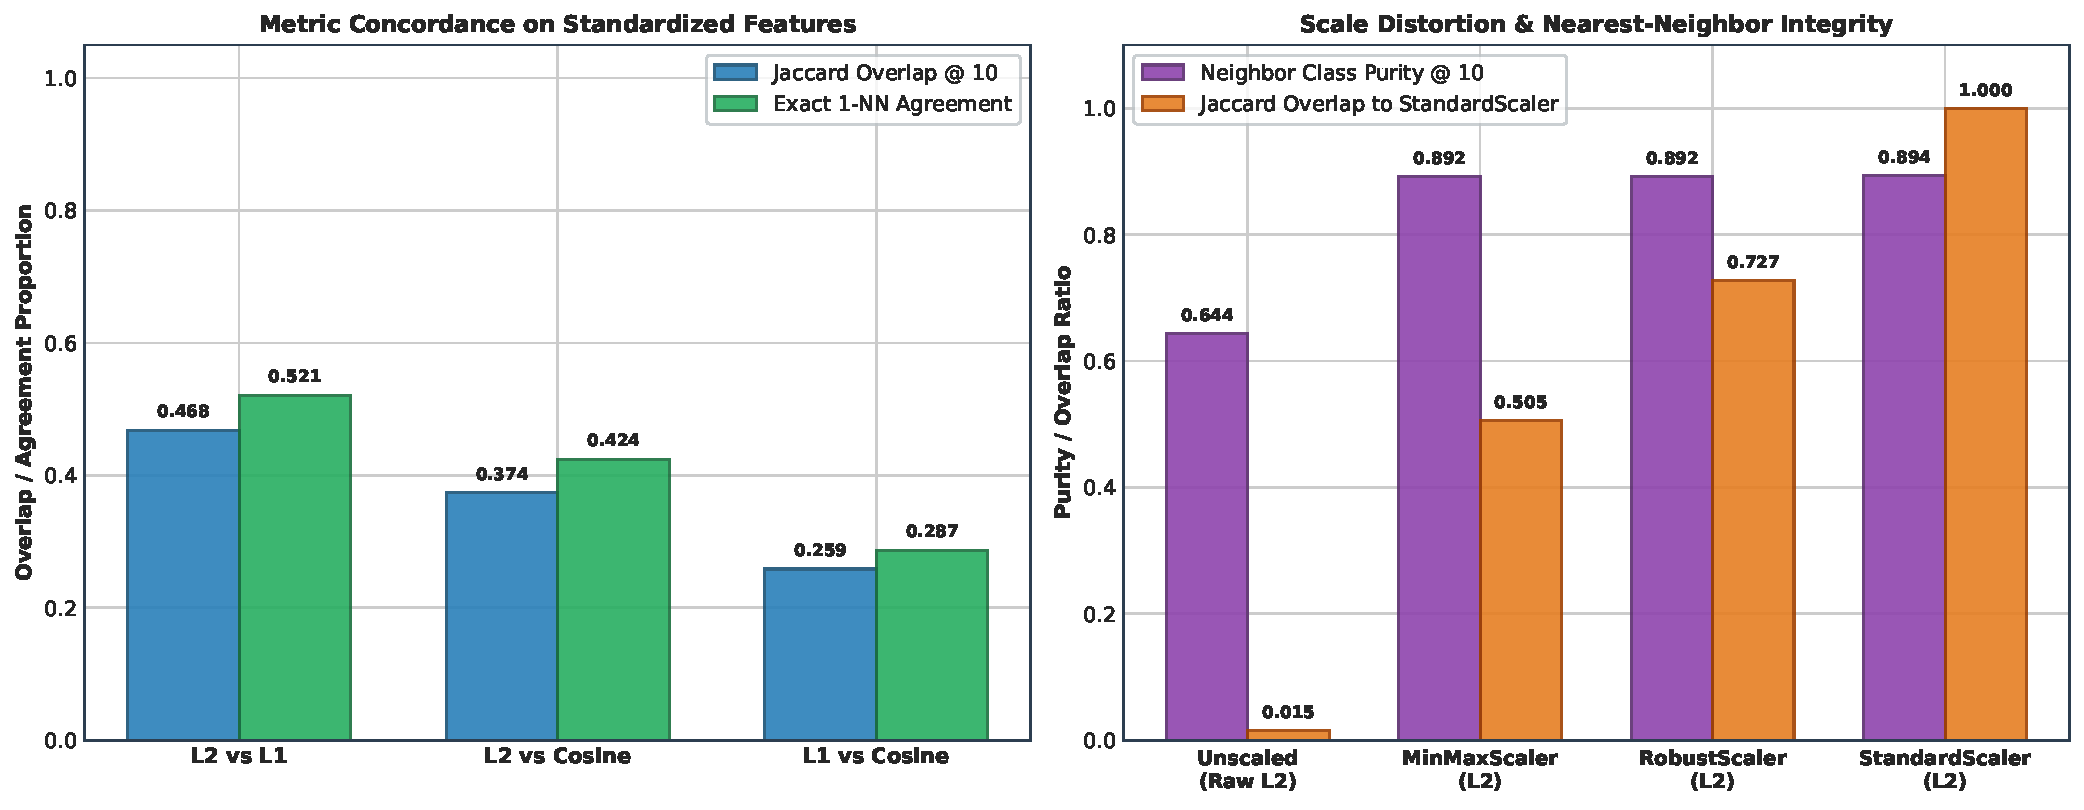
\includegraphics[width=0.88\linewidth]{fig08_similarity_distance_comparison}
    \caption{Nearest-neighbor concordance and scale distortion: (Left) Concordance across standardized $L_2, L_1$, and Cosine; (Right) Severe neighbor purity collapse ($\Delta = -0.2498$) on unscaled raw Euclidean distance.}
    \label{fig:dist_comp}
\end{figure}

On standardized features, Euclidean and Manhattan metrics yield nearly identical neighbor class purity ($89.37\%$ vs. $89.34\%$), despite sharing only a $46.76\%$ top-10 Jaccard overlap. On raw features, Euclidean overlap with standardized space collapses to $1.51\%$, and neighbor purity plunges by $\Delta = -0.2498$ (down to $64.39\%$). In raw space, query points match neighbors differing in \texttt{Area} by an average of only $35.76$ pixels, compared to $1{,}405.11$ pixels in standardized space. The $75.5\text{M}\times$ scale disparity forces raw Euclidean distance to function almost exclusively as a 1D pixel count sorter.

\subsection{Unsupervised Clustering Structure}
\label{subsec:res_clustering}

Table~\ref{tab:clustering} compares clustering algorithms on standardized features, evaluated alongside Figures~\ref{fig:kmeans_elbow} and~\ref{fig:clustering_pca}.

\begin{table}[htbp]
    \centering
    \small
    \caption{Unsupervised Clustering Performance Summary ($k=7$, Standardized Features).}
    \label{tab:clustering}
    \setlength{\tabcolsep}{4.5pt}
    \begin{tabularx}{\linewidth}{@{} >{\raggedright\arraybackslash}X cccccc @{}}
        \toprule
        \textbf{Clustering Algorithm} & \textbf{Instances} & \textbf{Clusters} & \textbf{Noise (\%)} & \textbf{Silhouette} & \textbf{ARI} & \textbf{NMI} \\
        \midrule
        \textbf{$k$-Means ($k=7$)} & $13{,}543$ & $7$ & $0.00\%$ & $0.3114$ & $\mathbf{0.6669}$ & $0.7124$ \\
        \textbf{Hierarchical Ward ($k=7$)} & $2{,}500$ & $7$ & $0.00\%$ & $0.2959$ & $0.6623$ & $\mathbf{0.7312}$ \\
        \textbf{DBSCAN ($\varepsilon=1.5, \text{min}=10$)} & $13{,}543$ & $2$ & $1.71\%$ & $\mathbf{0.5668}$ & $0.0343$ & $0.1554$ \\
        \bottomrule
    \end{tabularx}
\end{table}

\begin{figure}[htbp]
    \centering
    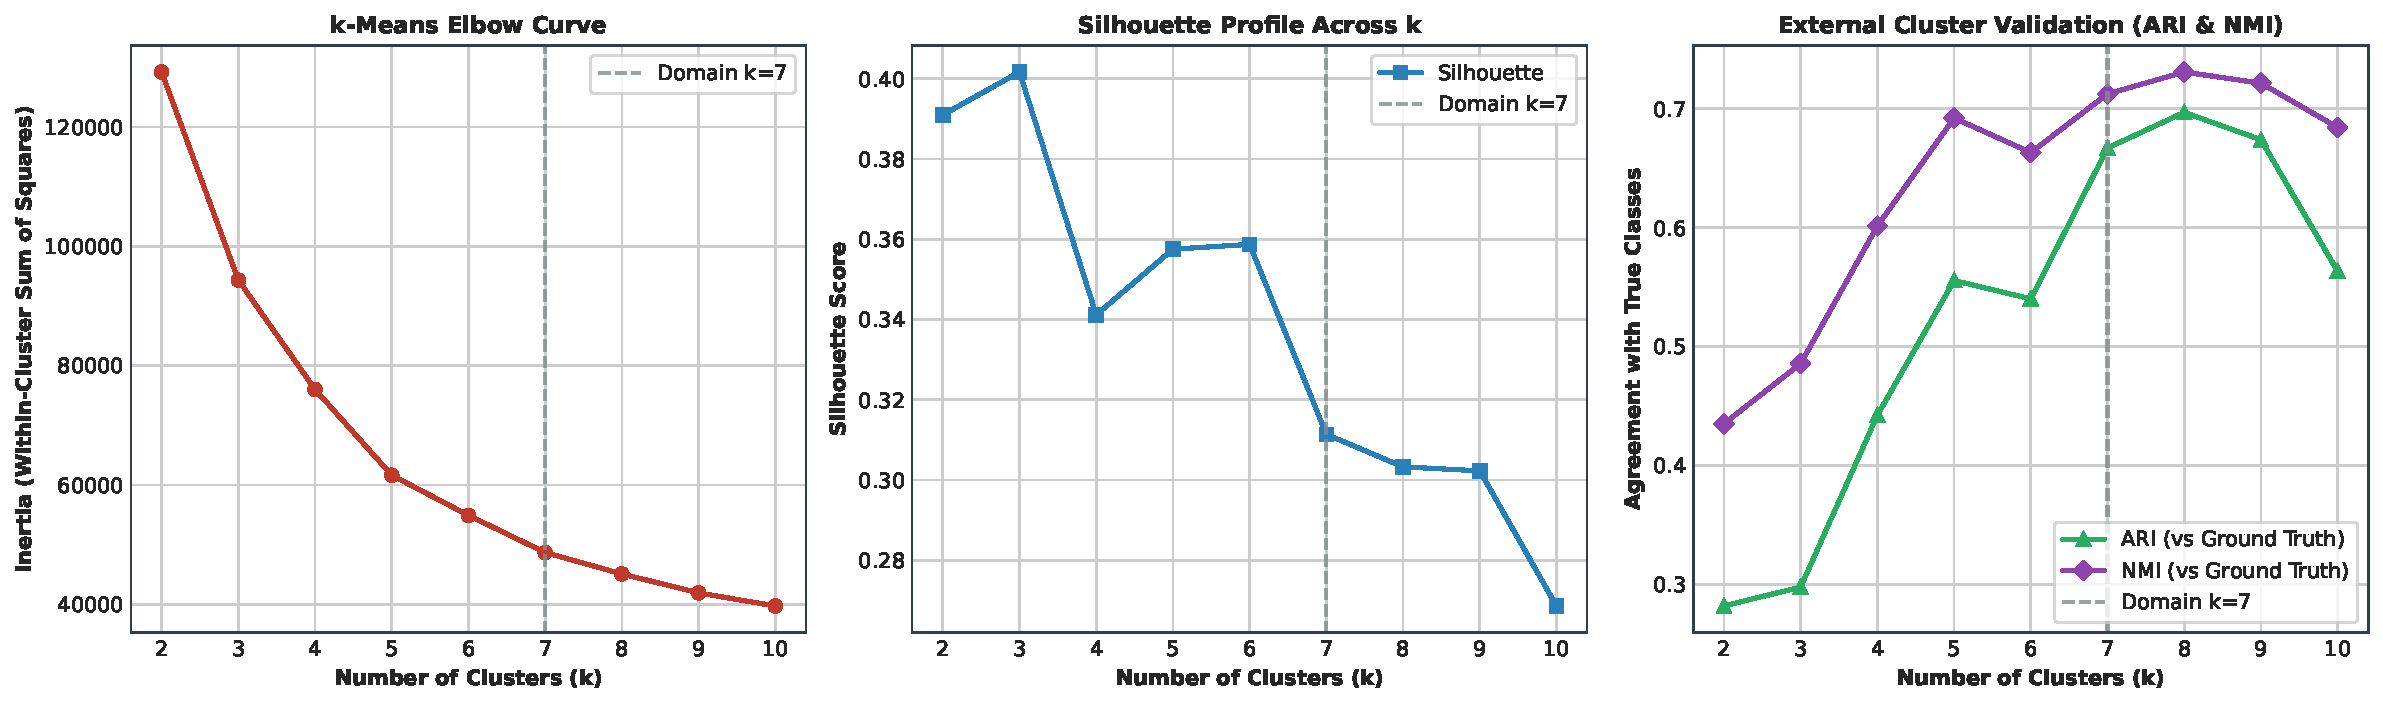
\includegraphics[width=0.88\linewidth]{fig09_kmeans_elbow_silhouette}
    \caption{$k$-Means clustering sweep across $k \in [2, 10]$: (Left) Inertia WCSS elbow; (Center) Silhouette score peaking at $k=3, 4$; (Right) External validation (ARI and NMI) maximizing at the domain cultivar specification $k=7$.}
    \label{fig:kmeans_elbow}
\end{figure}

\begin{figure}[htbp]
    \centering
    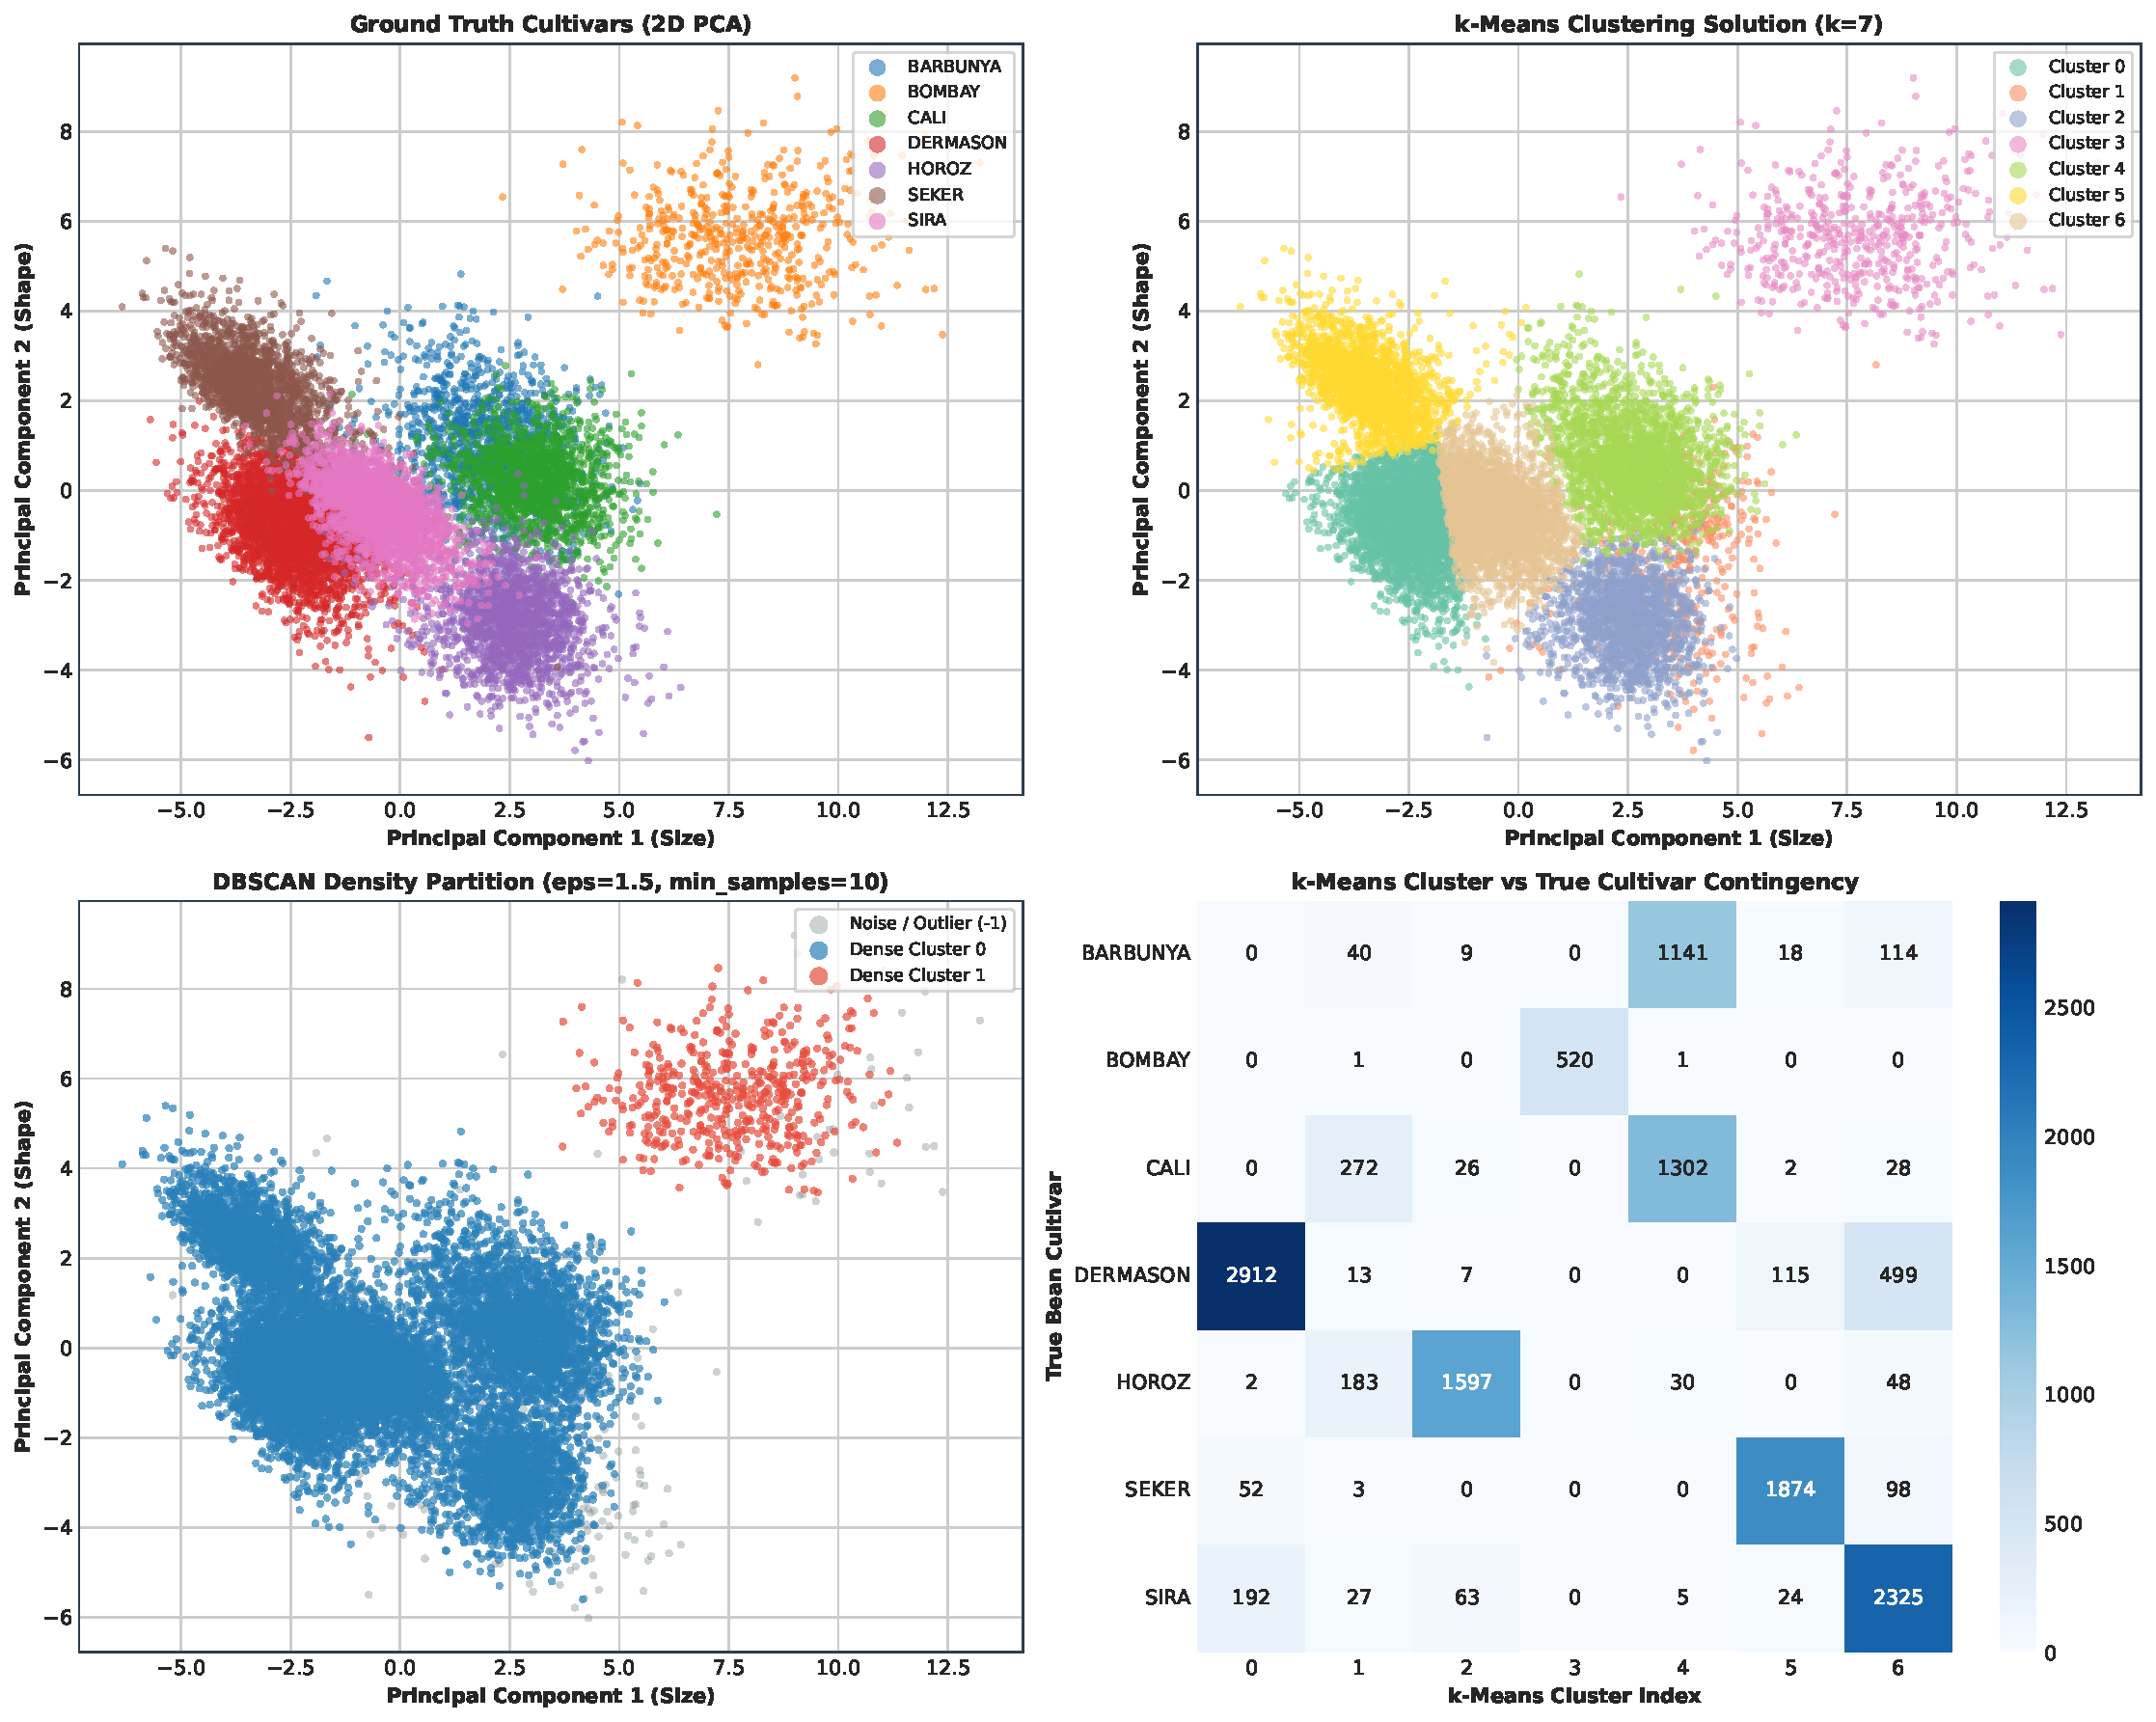
\includegraphics[width=0.88\linewidth]{fig10_clustering_comparison_pca}
    \caption{2D PCA projection of clustering partitions: Ground Truth vs. $k$-Means ($k=7$) vs. DBSCAN density partition, and contingency heatmap illustrating cultivar overlaps.}
    \label{fig:clustering_pca}
\end{figure}

The $k$-Means sweep shows geometric elbow inflections at $k = 3, 4$ (Silhouette $= 0.4074, 0.3541$). However, agreement with biological cultivars peaks at $k = 7$ ($\text{ARI} = 0.6669$, $\text{NMI} = 0.7124$). Hierarchical Ward linkage achieves closely congruent partitions ($\text{ARI} = 0.6623$). DBSCAN discovers exactly two dense clusters: Cluster 1 isolates $487$ \texttt{BOMBAY} grains with zero contamination, while Cluster 0 lumps the remaining six varieties into a single continuous density manifold ($12{,}825$ grains), proving that intermediate morphological transitions bridge non-\textit{Bombay} cultivars.

\subsection{Supervised Classification Performance}
\label{subsec:res_classification}

Table~\ref{tab:classification} summarizes model benchmark metrics on the stratified test split ($N_{\text{test}} = 2{,}709$), and Table~\ref{tab:per_class} reports per-class discrimination.

\begin{table}[htbp]
    \centering
    \small
    \caption{Supervised Classification Performance Across Four Algorithmic Paradigms.}
    \label{tab:classification}
    \setlength{\tabcolsep}{5pt}
    \begin{tabularx}{\linewidth}{@{} >{\raggedright\arraybackslash}X cccccc @{}}
        \toprule
        \textbf{Classifier} & \textbf{Accuracy} & \textbf{Macro-P} & \textbf{Macro-R} & \textbf{Macro-F1} & \textbf{W-F1} & \textbf{5-Fold CV} \\
        \midrule
        \textbf{$k$-Nearest Neighbors ($k=7$)} & $\mathbf{0.9118}$ & $\mathbf{0.9253}$ & $\mathbf{0.9224}$ & $\mathbf{0.9237}$ & $\mathbf{0.9119}$ & $\mathbf{0.9357}$ \\
        \textbf{Decision Tree (Tuned)} & $0.9070$ & $0.9220$ & $0.9204$ & $0.9211$ & $0.9071$ & $0.9236$ \\
        \textbf{Gaussian Naïve Bayes} & $0.8970$ & $0.9081$ & $0.9082$ & $0.9072$ & $0.8972$ & $0.9064$ \\
        \textbf{Rule-Based (Depth 4)} & $0.8158$ & $0.7363$ & $0.7889$ & $0.7520$ & $0.7839$ & $0.8072$ \\
        \bottomrule
    \end{tabularx}
\end{table}

\begin{table}[htbp]
    \centering
    \small
    \caption{Per-Class Precision, Recall, and F1-Scores on Test Split ($N_{\text{test}} = 2{,}709$).}
    \label{tab:per_class}
    \setlength{\tabcolsep}{3.2pt}
    \begin{tabular*}{\linewidth}{@{\extracolsep{\fill}} l cccccccc @{}}
        \toprule
        \multirow{2}{*}{\textbf{Cultivar}} & \multicolumn{2}{c}{\textbf{$k$-NN ($k=7$)}} & \multicolumn{2}{c}{\textbf{Decision Tree}} & \multicolumn{2}{c}{\textbf{Gaussian NB}} & \multicolumn{2}{c}{\textbf{Rule Classifier}} \\
        \cmidrule(lr){2-3} \cmidrule(lr){4-5} \cmidrule(lr){6-7} \cmidrule(lr){8-9}
        & \textbf{Rec} & \textbf{F1} & \textbf{Rec} & \textbf{F1} & \textbf{Rec} & \textbf{F1} & \textbf{Rec} & \textbf{F1} \\
        \midrule
        \texttt{BARBUNYA} & $0.8717$ & $0.8936$ & $0.9019$ & $0.9105$ & $0.7962$ & $0.8323$ & $0.0000$ & $0.0000$ \\
        \texttt{BOMBAY} & $\mathbf{1.0000}$ & $\mathbf{1.0000}$ & $\mathbf{1.0000}$ & $\mathbf{1.0000}$ & $\mathbf{1.0000}$ & $\mathbf{1.0000}$ & $\mathbf{1.0000}$ & $\mathbf{1.0000}$ \\
        \texttt{CALI} & $0.9387$ & $0.9175$ & $0.9325$ & $0.9184$ & $0.9233$ & $0.8892$ & $0.9755$ & $0.6752$ \\
        \texttt{DERMASON} & $0.9097$ & $0.9085$ & $0.9027$ & $0.9027$ & $0.8604$ & $0.8971$ & $0.9168$ & $0.9003$ \\
        \texttt{HOROZ} & $0.9355$ & $0.9482$ & $0.9194$ & $0.9421$ & $0.9462$ & $0.9501$ & $0.8737$ & $0.9233$ \\
        \texttt{SEKER} & $0.9360$ & $0.9406$ & $0.9384$ & $0.9304$ & $0.9360$ & $0.9291$ & $0.9310$ & $0.9322$ \\
        \texttt{SIRA} & $0.8653$ & $\mathbf{0.8571}$ & $0.8482$ & $\mathbf{0.8434}$ & $0.8956$ & $\mathbf{0.8528}$ & $0.8254$ & $\mathbf{0.8333}$ \\
        \bottomrule
    \end{tabular*}
\end{table}

\begin{figure}[htbp]
    \centering
    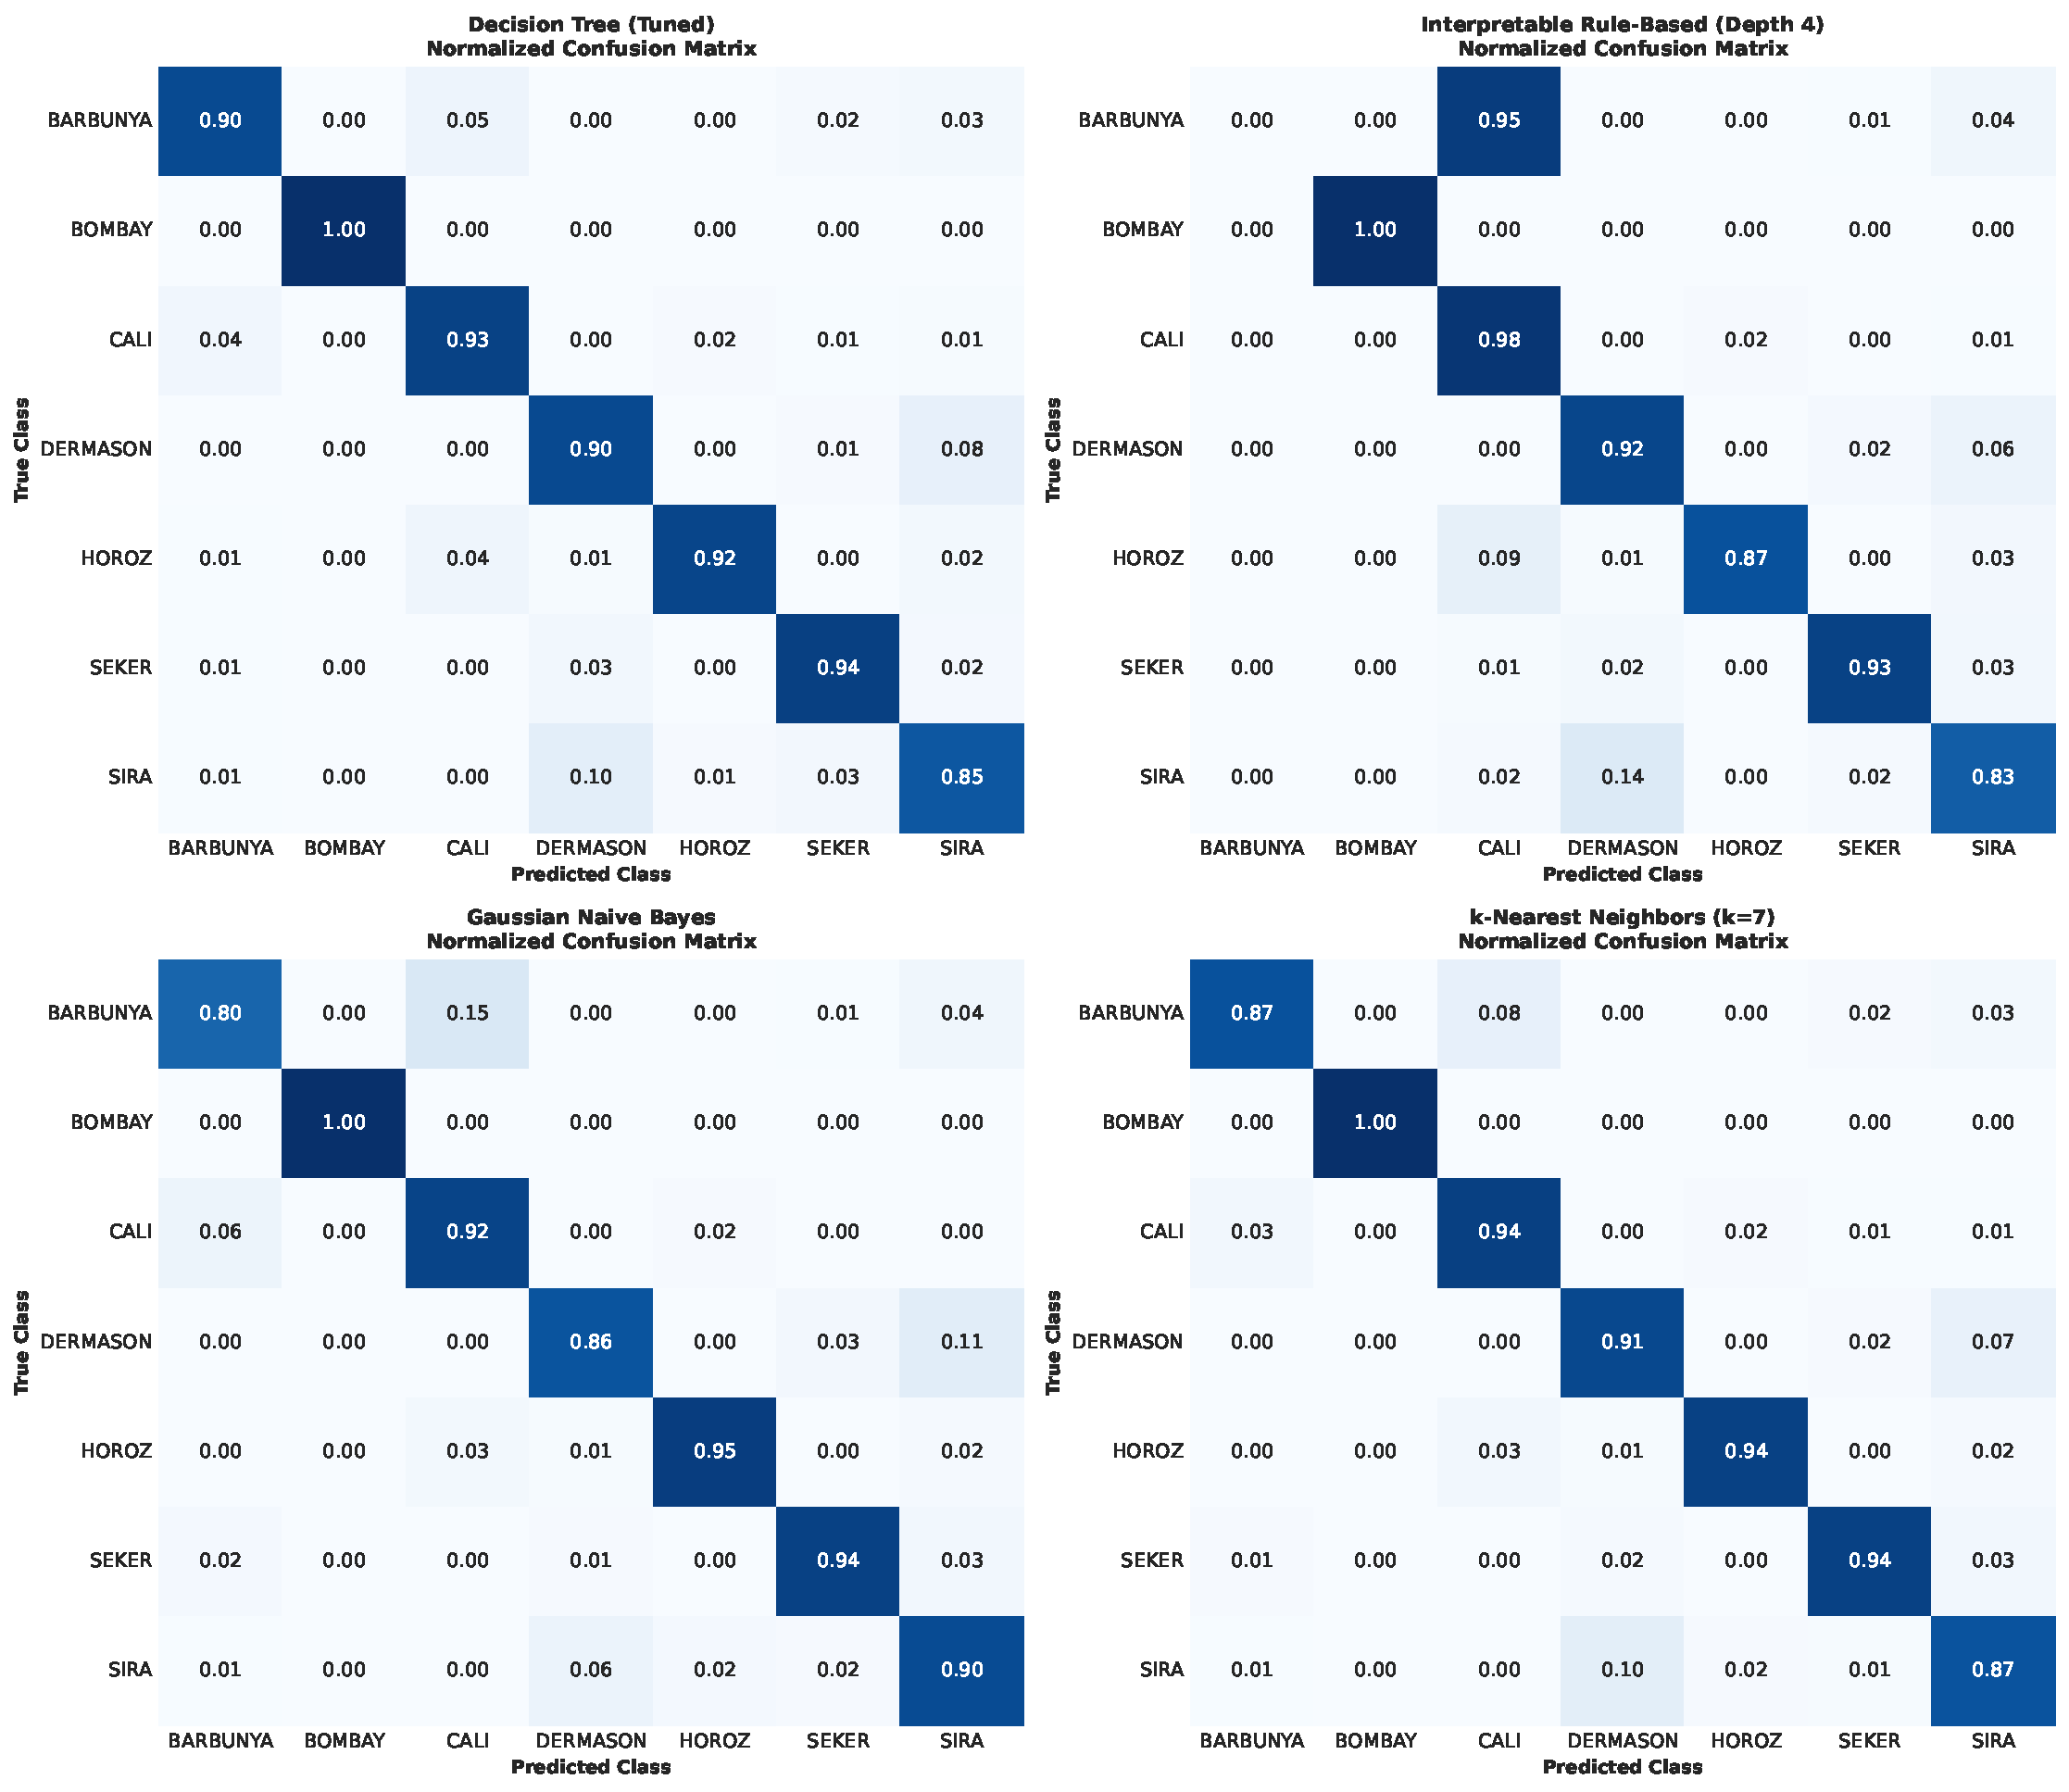
\includegraphics[width=0.88\linewidth]{fig11_classification_confusion_matrices}
    \caption{Normalized confusion matrices across four classification paradigms, illustrating perfect $100\%$ accuracy on \texttt{BOMBAY} and reciprocal confusion between \texttt{SIRA} and \texttt{DERMASON}.}
    \label{fig:conf_matrices}
\end{figure}

\texttt{BOMBAY} is classified with $100\%$ precision and recall across all models. Conversely, \texttt{SIRA} yields the lowest F1-score across all classifiers ($0.8434$--$0.8571$), misclassifying $63$ grains as \texttt{DERMASON} in $k$-NN and $68$ in Decision Tree. Figure~\ref{fig:conf_matrices} visualizes the normalized confusion matrices. In the depth-4 rule classifier, \texttt{BARBUNYA} achieves $0\%$ recall because its decision region is subsumed by \texttt{CALI} at coarse depths.

\subsection{Morphological Class Association Rules}
\label{subsec:res_association}

Table~\ref{tab:assoc_rules} lists top discovered Class Association Rules, and Figure~\ref{fig:assoc_scatter} charts Support vs. Confidence colored by Lift.

\begin{table}[htbp]
    \centering
    \small
    \caption{Top Discretized Morphological Class Association Rules Mined via FP-Growth.}
    \label{tab:assoc_rules}
    \setlength{\tabcolsep}{4.5pt}
    \begin{tabularx}{\linewidth}{@{} l >{\raggedright\arraybackslash}X cccc @{}}
        \toprule
        \textbf{Cultivar} & \textbf{Morphological Antecedent Rule} & \textbf{Support} & \textbf{Confidence} & \textbf{Lift} & \textbf{Conviction} \\
        \midrule
        \texttt{BARBUNYA} & $\text{Area}_{\text{High}} \land \text{Aspect}_{\text{Low}} \land \text{round}_{\text{Low}}$ & $0.0212$ & $\mathbf{0.9795}$ & $\mathbf{10.0345}$ & $44.07$ \\
        \texttt{CALI} & $\text{Area}_{\text{High}} \land \text{Aspect}_{\text{High}} \land \text{round}_{\text{Med}}$ & $0.0315$ & $0.7993$ & $6.6406$ & $4.38$ \\
        \texttt{HOROZ} & $\text{Area}_{\text{Med}} \land \text{Aspect}_{\text{High}} \land \text{round}_{\text{Low}}$ & $0.0589$ & $0.8515$ & $6.1999$ & $5.81$ \\
        \texttt{SEKER} & $\text{Area}_{\text{Med}} \land \text{Aspect}_{\text{Low}} \land \text{round}_{\text{High}}$ & $0.0399$ & $0.8257$ & $5.5167$ & $4.88$ \\
        \texttt{SIRA} & $\text{Area}_{\text{Med}} \land \text{Aspect}_{\text{Med}} \land \text{round}_{\text{Med}}$ & $0.0310$ & $0.9375$ & $4.8166$ & $12.89$ \\
        \texttt{DERMASON} & $\text{Area}_{\text{Low}} \land \text{Aspect}_{\text{Med}} \land \text{round}_{\text{High}}$ & $0.0509$ & $0.9801$ & $3.7433$ & $37.12$ \\
        \bottomrule
    \end{tabularx}
\end{table}

\begin{figure}[htbp]
    \centering
    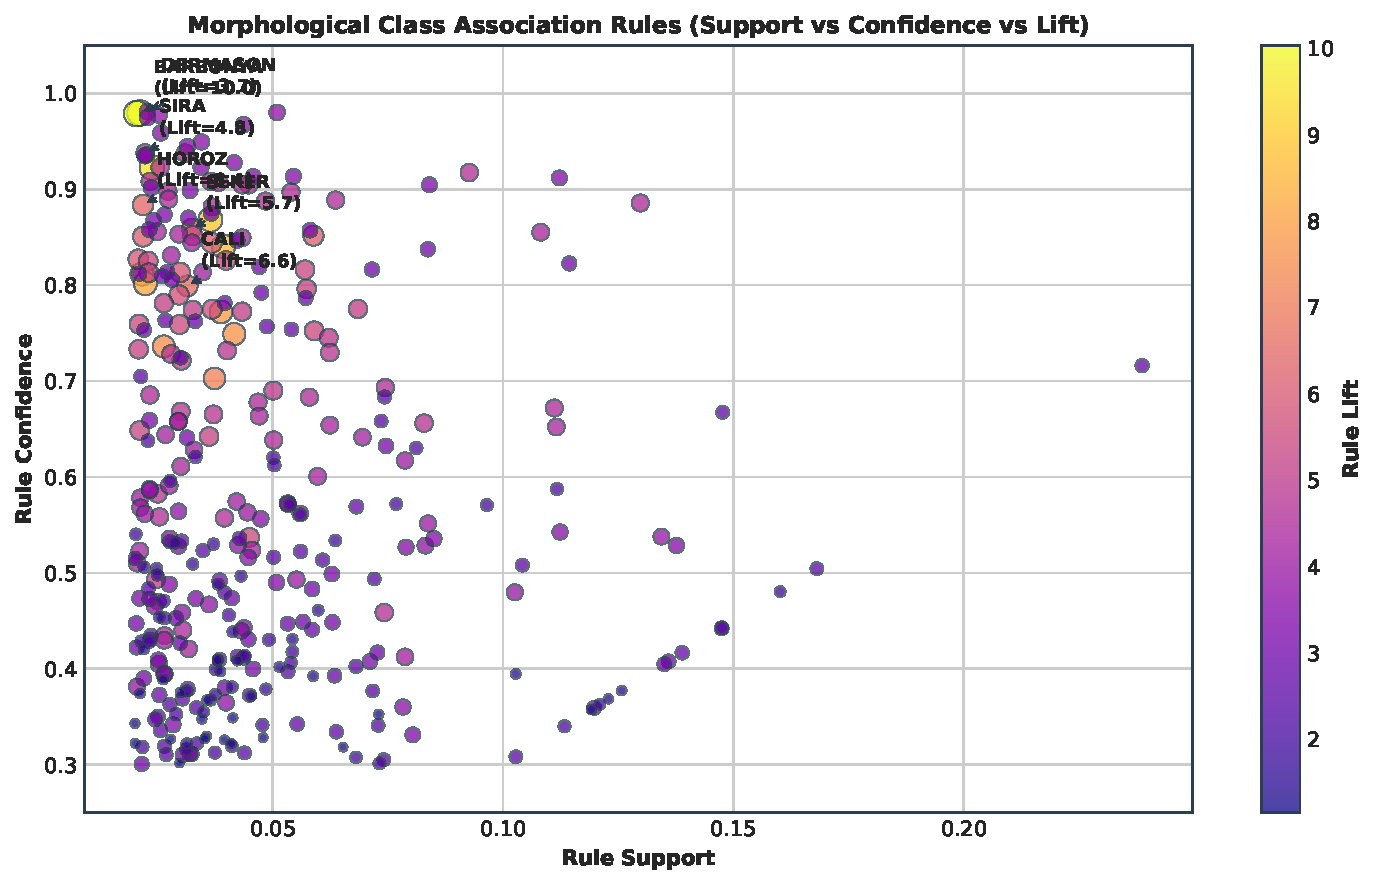
\includegraphics[width=0.84\linewidth]{fig12_association_rules_scatter}
    \caption{Morphological Class Association Rules: Support vs. Confidence colored by Lift, annotating biological signature rules across cultivars.}
    \label{fig:assoc_scatter}
\end{figure}

The rule $\{\text{Area}_{\text{High}} \land \text{Aspect}_{\text{Low}} \land \text{round}_{\text{Low}}\} \to \{\texttt{BARBUNYA}\}$ yields a maximum lift of $10.0345$ ($\text{Conf} = 97.95\%$), defining a distinct biological signature. In contrast, \texttt{DERMASON} rules achieve high confidence ($98.01\%$) but lower lift ($3.7433$), reflecting its high baseline prevalence ($26.18\%$).

\subsection{The Group 10 Data Mining Stress Test}
\label{subsec:res_stress_tests}

Table~\ref{tab:stress_summary} consolidates the results across all four controlled stress tests, evaluated alongside the signature robustness curves in Figures~\ref{fig:stress_missing}, \ref{fig:stress_outliers}, \ref{fig:stress_scaling}, and~\ref{fig:stress_features}. In Stress Test~1 (Figure~\ref{fig:stress_missing}), models degrade gracefully up to $10\%$ MCAR before median imputation buffers decision tree performance. In Stress Test~2 (Figure~\ref{fig:stress_outliers}), Decision Trees demonstrate near-complete outlier immunity while $k$-Means centroids collapse. In Stress Test~3 (Figure~\ref{fig:stress_scaling}), raw feature scaling collapses distance metrics while RobustScaler maintains clustering agreement under $10\%$ outlier contamination. Finally, in Stress Test~4 (Figure~\ref{fig:stress_features}), collinearity pruning boosts Gaussian Naïve Bayes accuracy by $+0.0136$ while preserving $k$-NN performance.

\begin{table}[htbp]
    \centering
    \footnotesize
    \caption{Consolidated Quantitative Performance Across the Four Stress-Test Experiments.}
    \label{tab:stress_summary}
    \setlength{\tabcolsep}{3.5pt}
    \begin{tabularx}{\linewidth}{@{} l >{\raggedright\arraybackslash}p{3.4cm} cccc >{\raggedright\arraybackslash}X @{}}
        \toprule
        \textbf{Experiment} & \textbf{Perturbation Level} & \textbf{DT F1} & \textbf{$k$-NN F1} & \textbf{GNB F1} & \textbf{KM ARI} & \textbf{Key Degradation Observation} \\
        \midrule
        \multirow{3}{*}{\textbf{SRQ1: Missing}} & Baseline ($0\%$ MCAR) & $0.9211$ & $0.9237$ & $0.9072$ & $0.6669$ & Pristine benchmark \\
        & $10\%$ MCAR (Median) & $0.8954$ & $0.9096$ & $0.8945$ & $0.6432$ & Graceful linear degradation \\
        & $30\%$ MCAR (Median) & $0.8563$ & $0.8710$ & $0.8840$ & $0.5620$ & Median buffers tree splits \\
        \midrule
        \multirow{3}{*}{\textbf{SRQ2: Outlier}} & Baseline ($0\%$ Outliers) & $0.9211$ & $0.9237$ & $0.9072$ & $0.6669$ & Clean uncorrupted geometry \\
        & $10\%$ Outliers ($+8\sigma$) & $0.9087$ & $0.9248$ & $0.8390$ & $0.4009$ & GNB / $k$-Means drop \\
        & $20\%$ Outliers ($+8\sigma$) & $\mathbf{0.9101}$ & $\mathbf{0.9246}$ & $0.8325$ & $\mathbf{0.2427}$ & DT robust ($\Delta = -0.0110$) \\
        \midrule
        \multirow{3}{*}{\textbf{SRQ3: Scaling}} & Raw Unscaled Data & $\mathbf{0.9197}$ & $\mathbf{0.7251}$ & $0.7669$ & $0.3881$ & $k$-NN / $k$-Means collapse \\
        & StandardScaler & $0.9211$ & $0.9237$ & $0.9072$ & $0.6669$ & Standardized benchmark \\
        & RobustScaler ($10\%$ Outlier) & $0.9087$ & $0.9267$ & $0.8390$ & $\mathbf{0.4926}$ & RobustScaler preserves ARI \\
        \midrule
        \multirow{3}{*}{\textbf{SRQ4: Features}} & All 16 Features (Collinear) & $0.9211$ & $0.9237$ & $\mathbf{0.9072}$ & $0.6669$ & Max VIF $= 317{,}671.59$ \\
        & Pruned 8 Features & $0.9144$ & $0.9238$ & $\mathbf{0.9208}$ & $0.4795$ & GNB gain $\Delta = +0.0136$ \\
        & PCA --- 2 Components & $0.8509$ & $0.8528$ & $0.8563$ & $0.6872$ & Fine boundary cues lost \\
        \bottomrule
    \end{tabularx}
\end{table}

\begin{figure}[htbp]
    \centering
    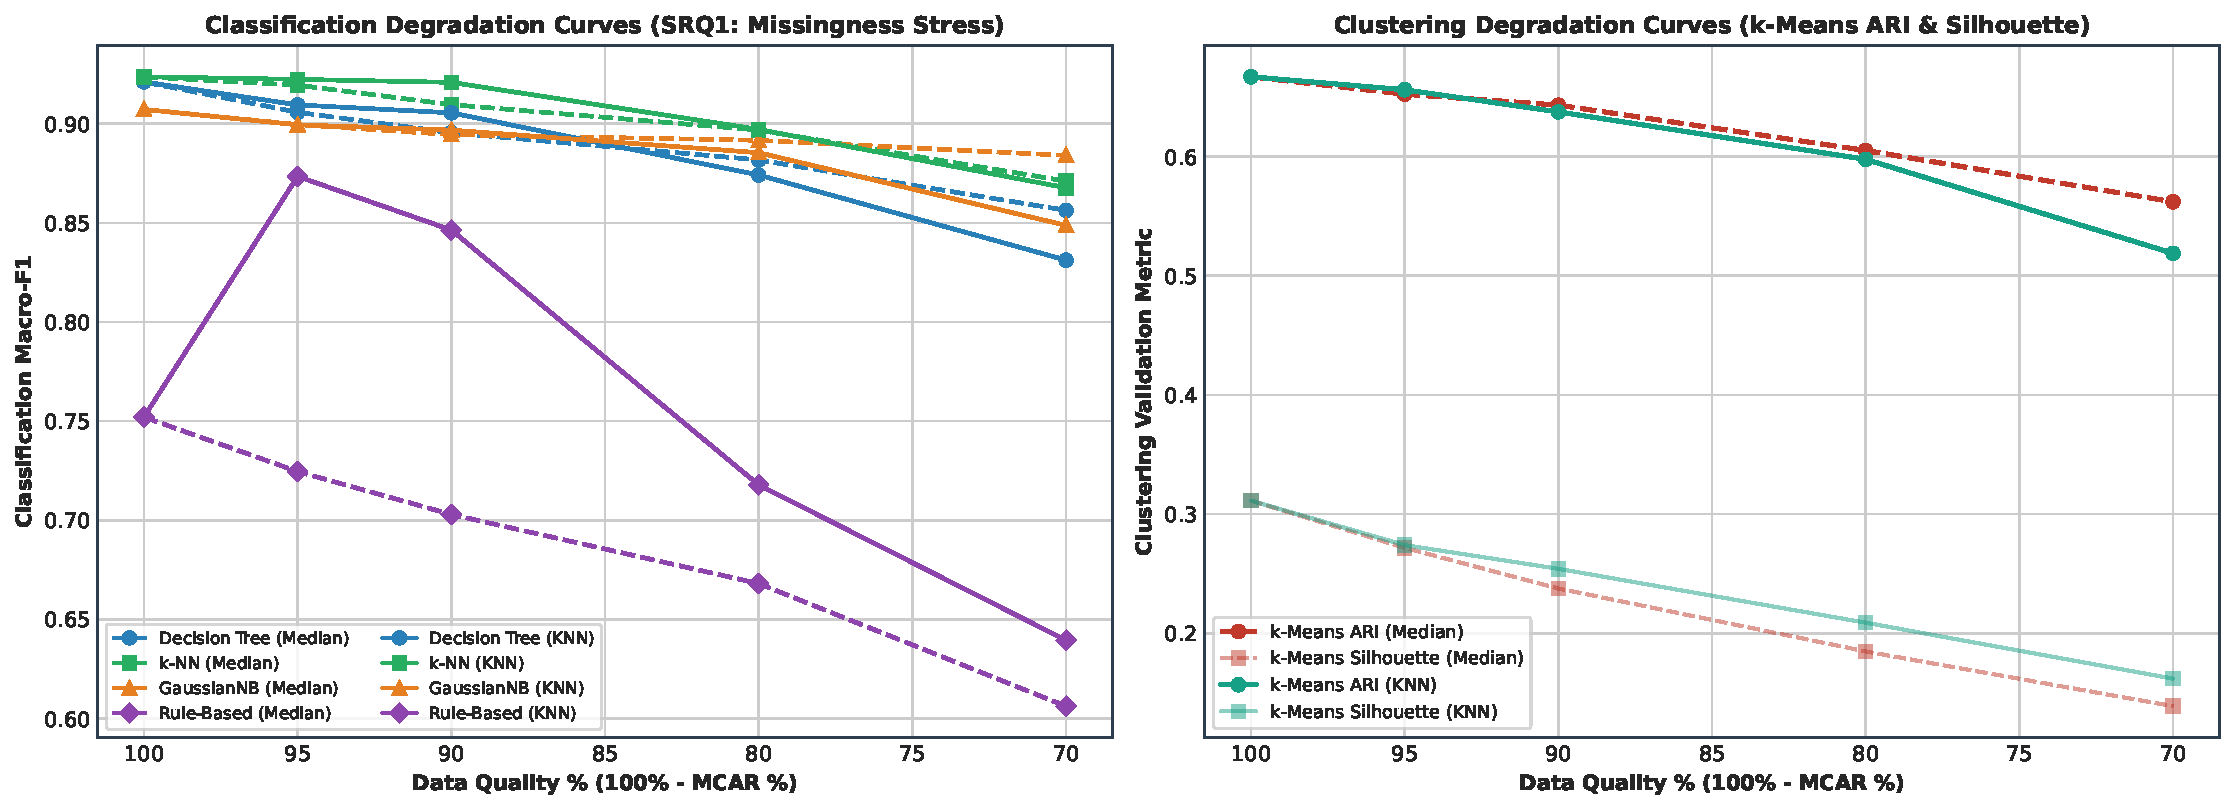
\includegraphics[width=0.88\linewidth]{fig13_robustness_curve_missing_data}
    \caption{Stress Test 1 (SRQ1): Classification Macro-F1 and $k$-Means ARI degradation curves across MCAR missingness levels ($0\%$--$30\%$) comparing Median vs. $k$-NN imputation.}
    \label{fig:stress_missing}
\end{figure}

\begin{figure}[htbp]
    \centering
    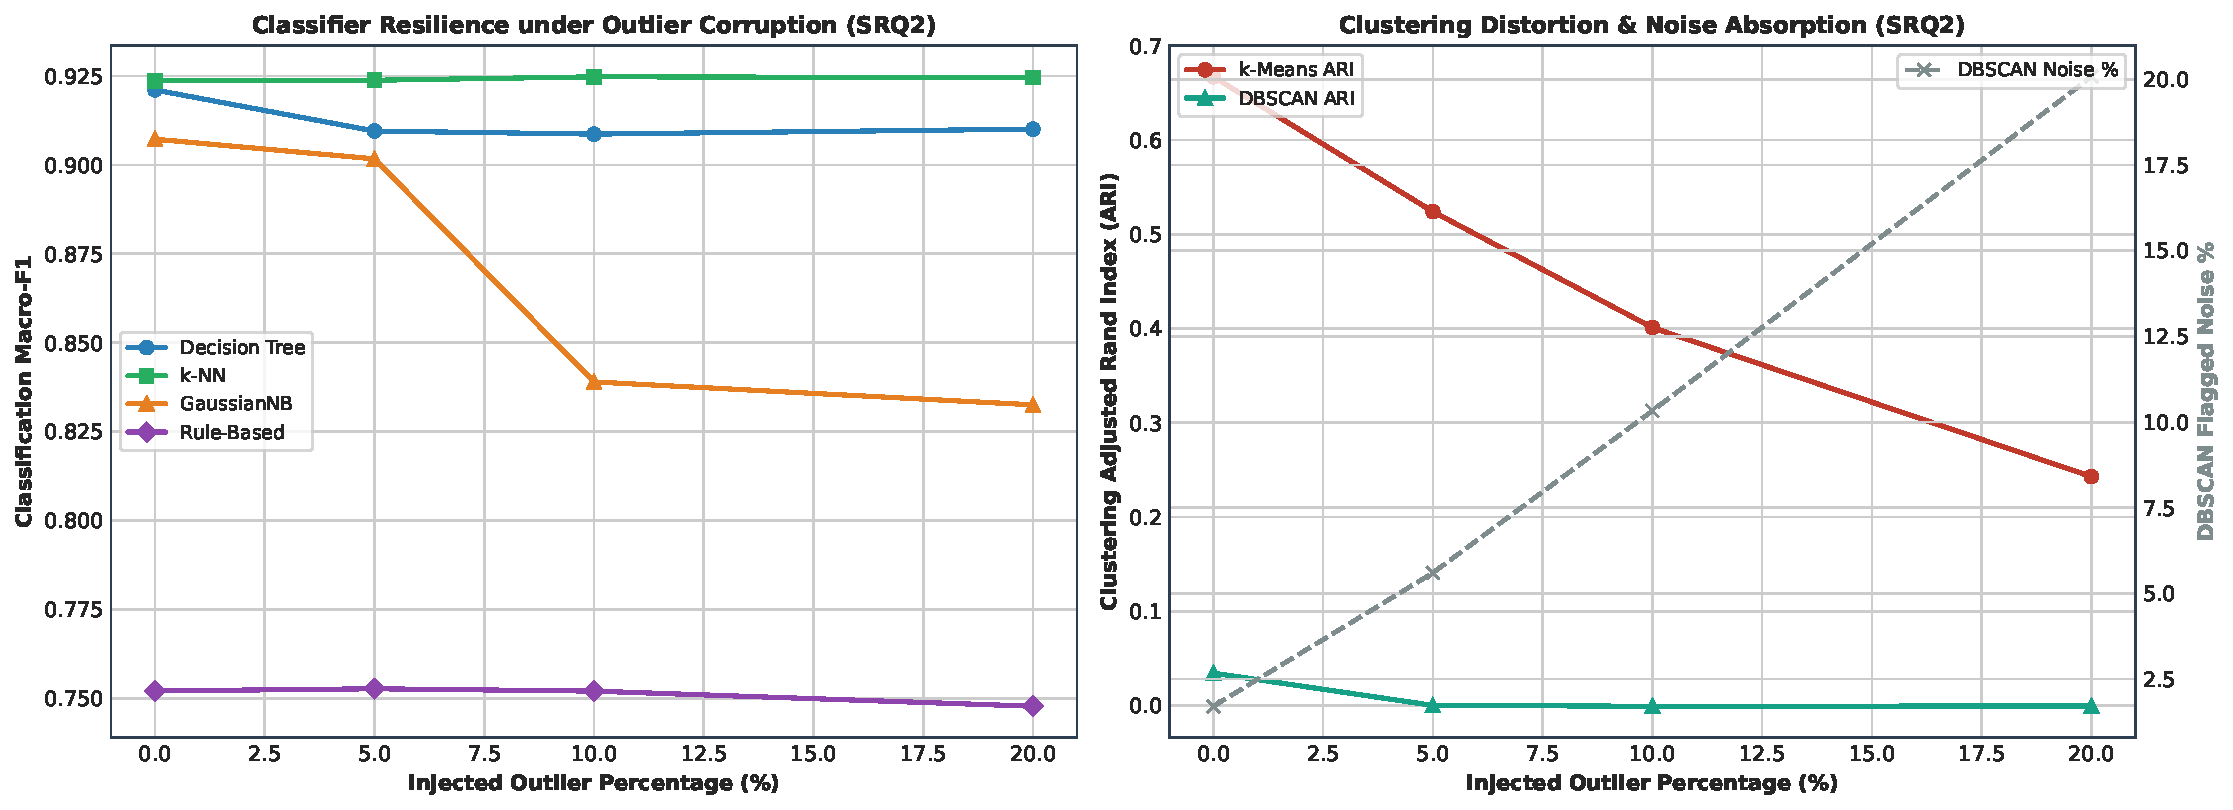
\includegraphics[width=0.88\linewidth]{fig14_robustness_curve_outliers}
    \caption{Stress Test 2 (SRQ2): Outlier injection robustness curves showing Decision Tree near-immunity vs. $k$-Means centroid collapse ($\Delta \text{ARI} = -0.4242$) and DBSCAN noise absorption.}
    \label{fig:stress_outliers}
\end{figure}

\begin{figure}[htbp]
    \centering
    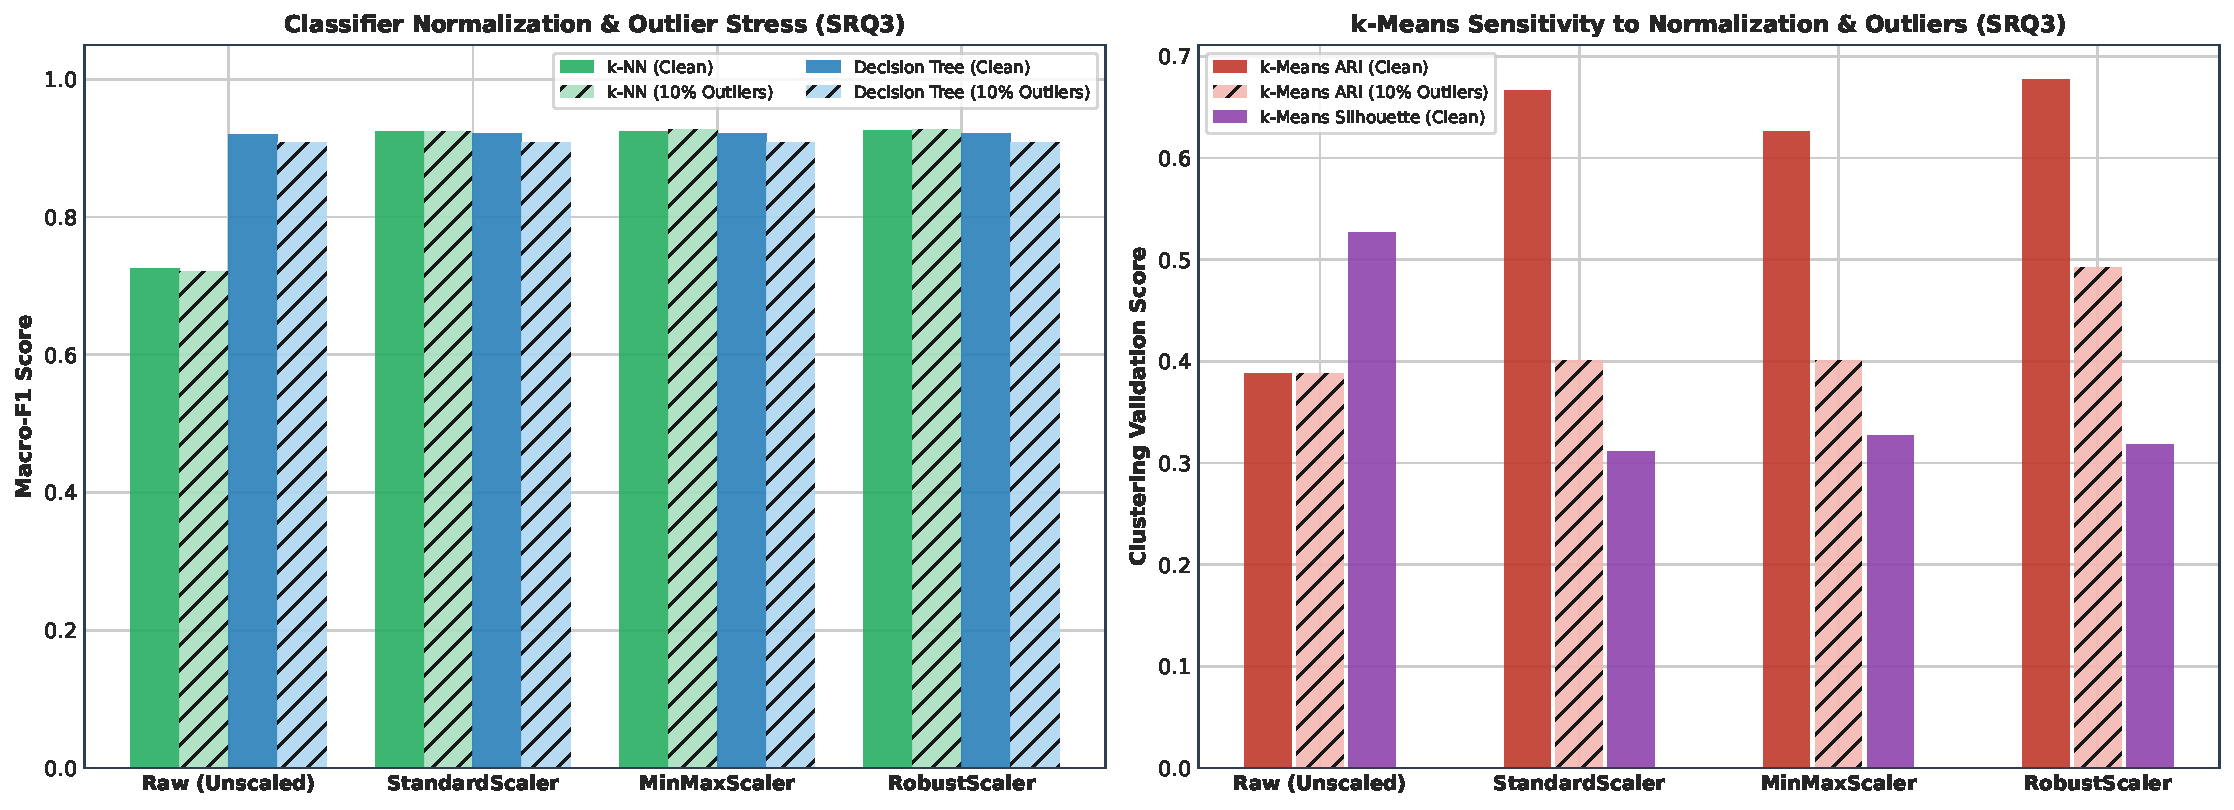
\includegraphics[width=0.88\linewidth]{fig15_scaling_sensitivity_stress}
    \caption{Stress Test 3 (SRQ3): Normalization sensitivity under clean and corrupted regimes, highlighting raw Euclidean distance collapse and RobustScaler outlier preservation.}
    \label{fig:stress_scaling}
\end{figure}

\begin{figure}[htbp]
    \centering
    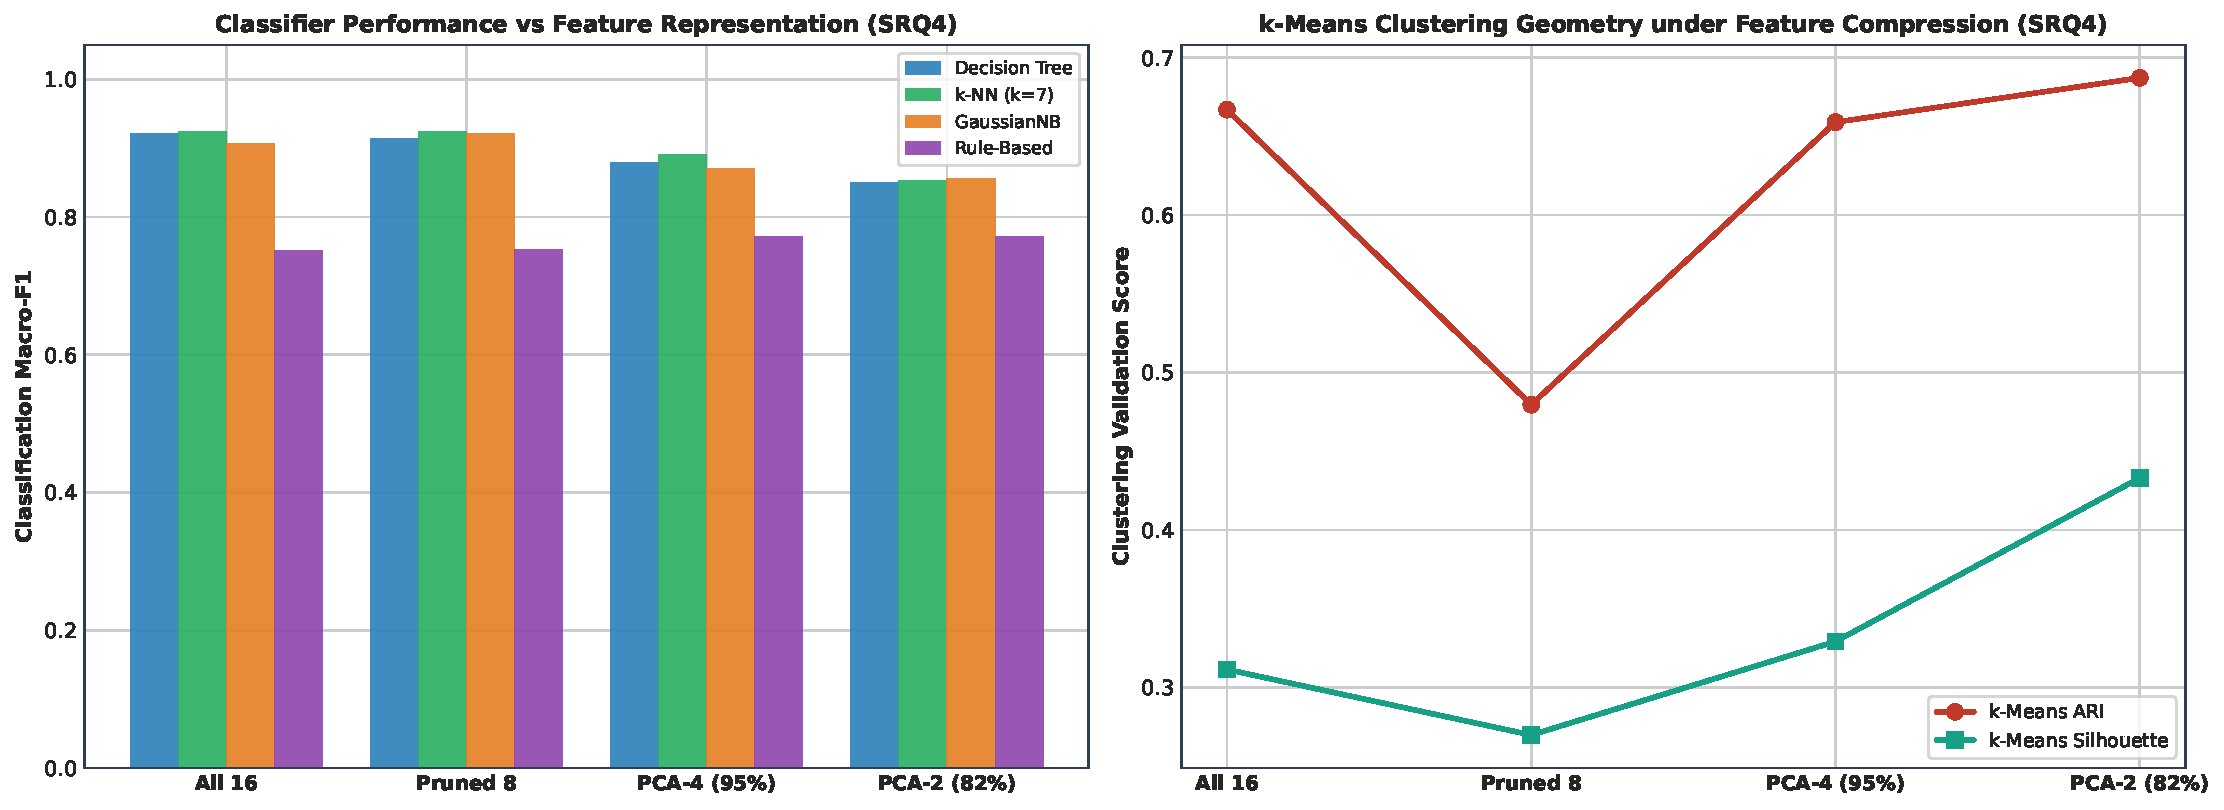
\includegraphics[width=0.88\linewidth]{fig16_feature_reduction_stress}
    \caption{Stress Test 4 (SRQ4): Dimensionality and collinearity stress showing Gaussian Naïve Bayes performance gain under collinearity pruning and PCA compression limits.}
    \label{fig:stress_features}
\end{figure}

% ==============================================================================
% SECTION 7: COMPARATIVE ANALYSIS
% ==============================================================================
\section{Comparative Analysis}
\label{sec:comparative_analysis}

Table~\ref{tab:master_comparison} presents the master comparative matrix synthesizing the behavior of all evaluated algorithmic paradigms under controlled stress.

\begin{table}[htbp]
    \centering
    \small
    \caption{Master Comparative Analysis Matrix Across Data Mining Paradigms Under Stress.}
    \label{tab:master_comparison}
    \setlength{\tabcolsep}{3.2pt}
    \begin{tabularx}{\linewidth}{@{} l >{\raggedright\arraybackslash}p{2.5cm} cccc >{\raggedright\arraybackslash}X @{}}
        \toprule
        \textbf{Model Algorithm} & \textbf{Paradigm} & \textbf{Clean F1} & \textbf{MCAR Drop} & \textbf{Outlier Drop} & \textbf{Scale Drop} & \textbf{Optimal Stress Regime} \\
        \midrule
        \textbf{Decision Tree} & Axis-Aligned Tree & $0.9211$ & $-0.0648$ & $\mathbf{-0.0110}$ & $\mathbf{-0.0014}$ & Scale-invariant; extreme outlier pipelines. \\
        \textbf{$k$-NN ($k=7$)} & Metric Space $k$-NN & $\mathbf{0.9237}$ & $-0.0560$ & $+0.0009$ & $\mathbf{-0.1985}$ & Normalized pipelines; moderate missingness. \\
        \textbf{Gaussian NB} & Probabilistic Bayes & $0.9072$ & $\mathbf{-0.0232}$ & $-0.0747$ & $-0.1403$ & De-correlated features; high missingness. \\
        \textbf{Rule Classifier} & Depth-Limited Rule & $0.7520$ & $-0.1458$ & $-0.0043$ & $0.0000$ & Human-auditable regulatory inspection. \\
        \textbf{$k$-Means} & Centroid WCSS & $0.6669^*$ & $-0.1049^*$ & $\mathbf{-0.4242^*}$ & $-0.2788^*$ & Pristine, spherical, outlier-free data. \\
        \bottomrule
        \multicolumn{7}{l}{\footnotesize $^*$Clustering performance evaluated via Adjusted Rand Index (ARI).}
    \end{tabularx}
\end{table}

\subsection{Algorithmic Mechanics of Divergence Under Stress}
\label{subsec:algorithmic_divergence}

The divergence in robustness across paradigms stems directly from their mathematical formulations:
\begin{itemize}[leftmargin=1.5em]
    \item \textbf{Decision Tree Outlier Immunity:} Tree splits evaluate rank-order inequalities ($x_j \le \theta$). Moving an outlier from $+2\sigma$ to $+8\sigma$ places it further into the existing partition without altering the threshold $\theta$, yielding near-zero degradation ($\Delta = -0.0110$, a $1.19\%$ relative decrease).
    \item \textbf{Decision Tree Scale Invariance:} Because rank order is preserved under strictly monotonic transformations, Decision Tree Macro-F1 is identical across Raw ($0.9197$) and Standardized ($0.9211$) regimes, with the tiny $0.0014$ difference attributable solely to floating-point split tie-breaking across the $75.5\text{M}\times$ scale disparity.
    \item \textbf{$k$-Means Centroid Collapse:} Because $k$-Means minimizes quadratic Euclidean errors $\sum \|\mathbf{x}_i - \boldsymbol{\mu}_k\|^2$, a single $+8\sigma$ outlier incurs $64\times$ the penalty of a $1\sigma$ point, forcefully dragging centroid coordinates into empty space and fracturing partitions ($\Delta \text{ARI} = -0.4242$).
    \item \textbf{Gaussian Naïve Bayes Collinearity Gain:} GNB multiplies likelihoods assuming independence. Pruning correlated size features eliminates redundant probability multiplication, improving Macro-F1 by $+0.0136$.
\end{itemize}

% ==============================================================================
% SECTION 8: FIVE HIGH-IMPACT FINDINGS
% ==============================================================================
\section{Five High-Impact Interesting Findings}
\label{sec:findings}

We formalize our five most significant empirical discoveries using the structured Observation--Evidence--Interpretation framework:

\subsection{Finding 1: The 100\% BOMBAY Outlier Paradox and Zero-Contamination Isolation}
\begin{itemize}[leftmargin=1.5em]
    \item \textbf{Observation:} Exactly $522$ out of $522$ \texttt{BOMBAY} beans ($100.0\%$) are flagged as statistical IQR outliers in global univariate auditing, yet \texttt{BOMBAY} achieves perfect $100\%$ classification accuracy across every tested model.
    \item \textbf{Evidence:} Table~\ref{tab:data_quality} records $522/522$ \texttt{BOMBAY} instances exceeding the global IQR threshold ($99{,}031.25$ pixels). Table~\ref{tab:per_class} confirms Precision $= 1.000$, Recall $= 1.000$, and F1 $= 1.000$ across all classifiers. DBSCAN (Table~\ref{tab:clustering}) isolates $487$ \texttt{BOMBAY} grains into a dedicated cluster with zero contamination.
    \item \textbf{Interpretation:} Global univariate outlier filters assume unimodal distributions. Because \textit{Bombay} is biologically a giant cultivar (mean Area $= 173{,}485.06$ pixels vs. overall median $= 44{,}580.00$ pixels), its entire subpopulation lies beyond the global whisker. What global statistics flag as ``noise'' is pure, biologically separable class signal.
\end{itemize}

\subsection{Finding 2: Raw Euclidean Distance Collapse and Area Hijacking}
\begin{itemize}[leftmargin=1.5em]
    \item \textbf{Observation:} Unscaled Euclidean distance collapses into a 1D pixel count sort, destroying nearest-neighbor class purity.
    \item \textbf{Evidence:} Table~\ref{tab:similarity} demonstrates that raw Euclidean distance shares only a $0.0151$ ($1.51\%$) top-10 Jaccard overlap with standardized space. Neighbor purity plunges by $\Delta = -0.2498$ (from $89.37\%$ to $64.39\%$), and $k$-NN Macro-F1 collapses by $\Delta = -0.1985$ (Table~\ref{tab:master_comparison}).
    \item \textbf{Interpretation:} The $75.5\text{M}\times$ scale disparity between \texttt{Area} ($[20{,}420, 254{,}616]$) and \texttt{ShapeFactor2} ($[0.000564, 0.003666]$) forces squared differences in \texttt{Area} to contribute $> 99.9\%$ of total distance, discarding circularity and elongation cues.
\end{itemize}

\subsection{Finding 3: Naïve Bayes Performance Inversion Under Collinearity Pruning}
\begin{itemize}[leftmargin=1.5em]
    \item \textbf{Observation:} Pruning half the predictive features improves Gaussian Naïve Bayes classification accuracy.
    \item \textbf{Evidence:} Table~\ref{tab:stress_summary} records GNB Macro-F1 increasing from $0.9072$ on all 16 features (max VIF $= 317{,}671.59$) to $\mathbf{0.9208}$ on the pruned 8-feature subset (max VIF $= 18.44$), producing a net gain of $\Delta = +0.0136$.
    \item \textbf{Interpretation:} Pairwise correlations exceeding $r > 0.98$ violate GNB's conditional independence assumption, multiplying size evidence redundantly. Removing collinear dimensions restores the theoretical validity of GNB likelihood products.
\end{itemize}

\subsection{Finding 4: Decision Tree Invariance to Extreme Outlier Corruption}
\begin{itemize}[leftmargin=1.5em]
    \item \textbf{Observation:} Decision Trees maintain near-perfect classification performance under severe outlier contamination, whereas $k$-Means clustering collapses catastrophically.
    \item \textbf{Evidence:} Table~\ref{tab:stress_summary} shows Decision Tree Macro-F1 dropping by only $1.10$ percentage points ($\Delta = -0.0110$, a $1.19\%$ relative drop from $0.9211$ to $0.9101$ at $20\%$ outliers), whereas $k$-Means ARI collapses by $\Delta = -0.4242$ (from $0.6669$ to $0.2427$).
    \item \textbf{Interpretation:} Decision tree split thresholds evaluate rank-order inequalities ($x_j \le \theta$). Shifted $+8\sigma$ outliers simply populate the extreme leaf node without displacing the threshold $\theta$.
\end{itemize}

\subsection{Finding 5: High-Lift Signatures vs. Prevalence Dilution in Association Rules}
\begin{itemize}[leftmargin=1.5em]
    \item \textbf{Observation:} Discretized FP-Growth discovers asymmetric rule lift across cultivars, establishing high-lift signatures for distinctive varieties and low-lift rules for overlapping varieties.
    \item \textbf{Evidence:} Table~\ref{tab:assoc_rules} documents $\{\text{Area}_{\text{High}} \land \text{Aspect}_{\text{Low}} \land \text{round}_{\text{Low}}\} \to \{\texttt{BARBUNYA}\}$ achieving $\text{Lift} = 10.0345$ ($\text{Conf} = 97.95\%$) and $\{\text{Area}_{\text{Med}} \land \text{Aspect}_{\text{High}} \land \text{round}_{\text{Low}}\} \to \{\texttt{HOROZ}\}$ achieving $\text{Lift} = 6.1999$, compared to \texttt{DERMASON} rules yielding lift below $3.75$.
    \item \textbf{Interpretation:} High-lift rules identify specific combinations of morphological tertiles unique to a cultivar. Low-lift rules reflect baseline cultivar prevalence boundaries and continuous morphological overlap between \texttt{DERMASON} and \texttt{SIRA}.
\end{itemize}

% ==============================================================================
% SECTION 9: LIMITATIONS
% ==============================================================================
\section{Limitations}
\label{sec:limitations}

While our findings provide actionable engineering guidance, several experimental limitations must be noted:
\begin{enumerate}[leftmargin=1.5em]
    \item \textbf{Controlled Laboratory Imagery:} The dataset features high-contrast segmentation against uniform backgrounds under controlled lighting. It lacks color, surface pigmentation, and real-world field occlusions (such as broken grains or soil debris).
    \item \textbf{Missingness Assumptions:} We injected Missing Completely at Random (MCAR) values. In industrial sorting, missingness is often Missing Not at Random (MNAR), such as dark grains causing sensor dropout.
    \item \textbf{Subsampling in Hierarchical Clustering:} Agglomerative Ward clustering was executed on a stratified subsample of $n = 2{,}500$ to prevent quadratic memory exhaustion ($O(N^2)$). While stratified sampling preserves cultivar proportions, it may miss rare boundary micro-clusters.
\end{enumerate}

% ==============================================================================
% SECTION 10: CONCLUSION & FUTURE WORK
% ==============================================================================
\section{Conclusion and Future Work}
\label{sec:conclusion}

This research provides a rigorous empirical stress test of data mining pipelines under controlled degradation. We conclude with direct, evidence-backed answers to our core research questions:

\subsection{Synthesis of Research Questions}
\label{subsec:synthesis_rq}

\begin{itemize}[leftmargin=1.5em]
    \item \textbf{Answer to RQ1 \& RQ2:} Dry bean morphology is governed by two dominant physical axes: grain size (PC1, $55.55\%$ variance) and elongation (PC2, $26.36\%$ variance), which cumulatively explain $81.91\%$ of total variance ($4$ components reach $95.00\%$). Global feature ranking demonstrates that primary size attributes exhibit the highest raw association with cultivars (\texttt{Area}, ANOVA $F = 29{,}014.84$, $\text{MI} = 1.0353$; \texttt{ConvexArea}, ANOVA $F = 28{,}960.45$; \texttt{Perimeter}, $\text{MI} = 1.0551$). However, due to extreme pairwise collinearity ($r > 0.96$), derived scale-invariant shape factors (\texttt{ShapeFactor2}, \texttt{ShapeFactor1}, and \texttt{AspectRation}) provide essential complementary discrimination once collinear geometric duplicates are pruned.
    \item \textbf{Answer to RQ3:} Three natural macro-clusters emerge: giant grains (\texttt{BOMBAY}, completely separated), circular grains (\texttt{SEKER}), and elongated grains. Severe morphological overlap occurs between \texttt{SIRA} and \texttt{DERMASON} (accounting for $> 65\%$ of all classification errors) and between \texttt{BARBUNYA} and \texttt{CALI}.
    \item \textbf{Answer to RQ4:} For supervised deployment under sensor degradation, \textbf{$k$-Nearest Neighbors ($k=7$) paired with RobustScaler} delivers the highest overall performance (Macro-F1 $= 0.9237$) and strongest resilience across moderate missingness. Where computational simplicity or outlier immunity is paramount, \textbf{Decision Trees} provide unmatched scale invariance and outlier robustness.
    \item \textbf{Answer to SRQ1--SRQ4:} Pipelines degrade gracefully up to $10\%$ MCAR missingness ($F_1 > 0.89$), with Median imputation buffering tree models effectively. Decision Trees exhibit complete resilience to $+8\sigma$ outliers ($\Delta = -0.0110$), whereas $k$-Means collapses catastrophically ($\Delta \text{ARI} = -0.4242$). Raw unscaled Euclidean distance collapses into a 1D pixel sort ($\Delta = -0.1985$), which RobustScaler successfully prevents. Pruning collinear features directly improves Gaussian Naïve Bayes Macro-F1 by $+0.0136$.
\end{itemize}

\subsection{Practical Recommendations for Agricultural Pipelines}
\label{subsec:recommendations}

Industrial sorting facilities should deploy a hybrid architecture: (1) apply RobustScaler preprocessing to prevent scale hijacking and outlier inflation; (2) utilize pruned 8-feature representations to eliminate collinearity; and (3) combine $k$-NN for high-confidence primary sorting with shallow Decision Tree cascades for rapid, outlier-immune reject gates. Future extensions will examine multi-spectral imagery and deep learning robustness under optical noise.

% ==============================================================================
% REFERENCES
% ==============================================================================
\newpage
\bibliographystyle{unsrtnat}
\bibliography{references}

\end{document}
